\section{农业生产全过程数字化技术}

\begin{frame}
    \frametitle{农业数据采集}
    我国农业生产存在人工成本迅速增加；生产规模小；方式落后；效率效益低等问题。发展智慧农业，通过电脑替代人脑，机器替代人力可以很好的解决这些问题。首先需要建设人机协同的天空地一体化数据信息采集体系，获取农业数字化信息。

    采集方法：
    \begin{figure}[htpb]
        \centering
        \setcounter{subfigure}{0}
        \subfloat[温湿度传感器]{
\includegraphics[height=3cm]{温湿度传感器}}\hfill
        \subfloat[光照传感器]{
\includegraphics[height=3cm]{光照传感器}}\hfill
        \subfloat[土壤温湿度传感器]{
\includegraphics[height=3cm]{土壤温湿度传感器}}\hfill
        \subfloat[CO$_2$浓度传感器]{
\includegraphics[height=3cm]{CO2浓度传感器}}
    \end{figure}
    
    

\end{frame}


\subsection{3S技术}

\begin{frame}
    \frametitle{3S技术}
    3S技术是全球卫星导航系统(Global Navigation Satellite System，GNSS)、遥感技术(Remote sensing，RS)和地理信息系统(Geography information systems，GIS)的统称，是空间技术、传感器技术、卫星定位与导航技术和计算机技术、通讯技术相结合，多学科高度集成的对空间信息进行采集、处理、管理、分析、表达、传播和应用的现代信息技术 。

    \bigskip
    在农业领域，“3S”技术可以为现代农业建立与之相适应的地理信息系统，为农业的规划、设计、管理、生产、决策过程提供更为精确的信息，在农业领域应用优势非常明显。上世纪80年代起，“3S”技术在我国农业领域开始有所应用，历经多年发展，产生了巨大的经济和社会效益，成为推动“数字农业”发展的重要手段。

\end{frame}

\begin{frame}
    \frametitle{全球卫星导航系统 GNSS}
    \begin{figure}[htpb]
        \centering
        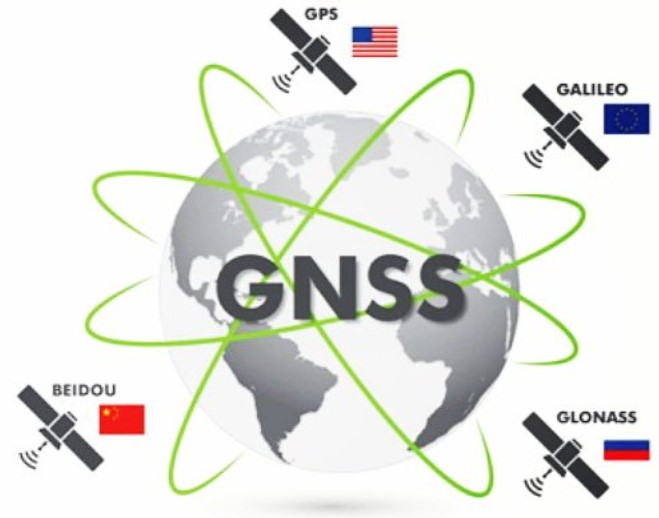
\includegraphics[height=.4\linewidth]{images/GNSS}
        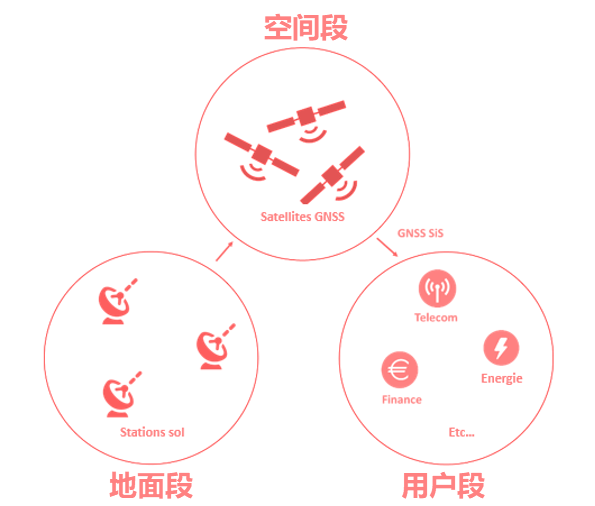
\includegraphics[height=.4\linewidth]{images/GNSS组成}
    \end{figure}
\end{frame}


\begin{frame}
    \frametitle{智能手机---卫星导航大规模在社会个人普及}
    \begin{figure}[htpb]
        \centering
        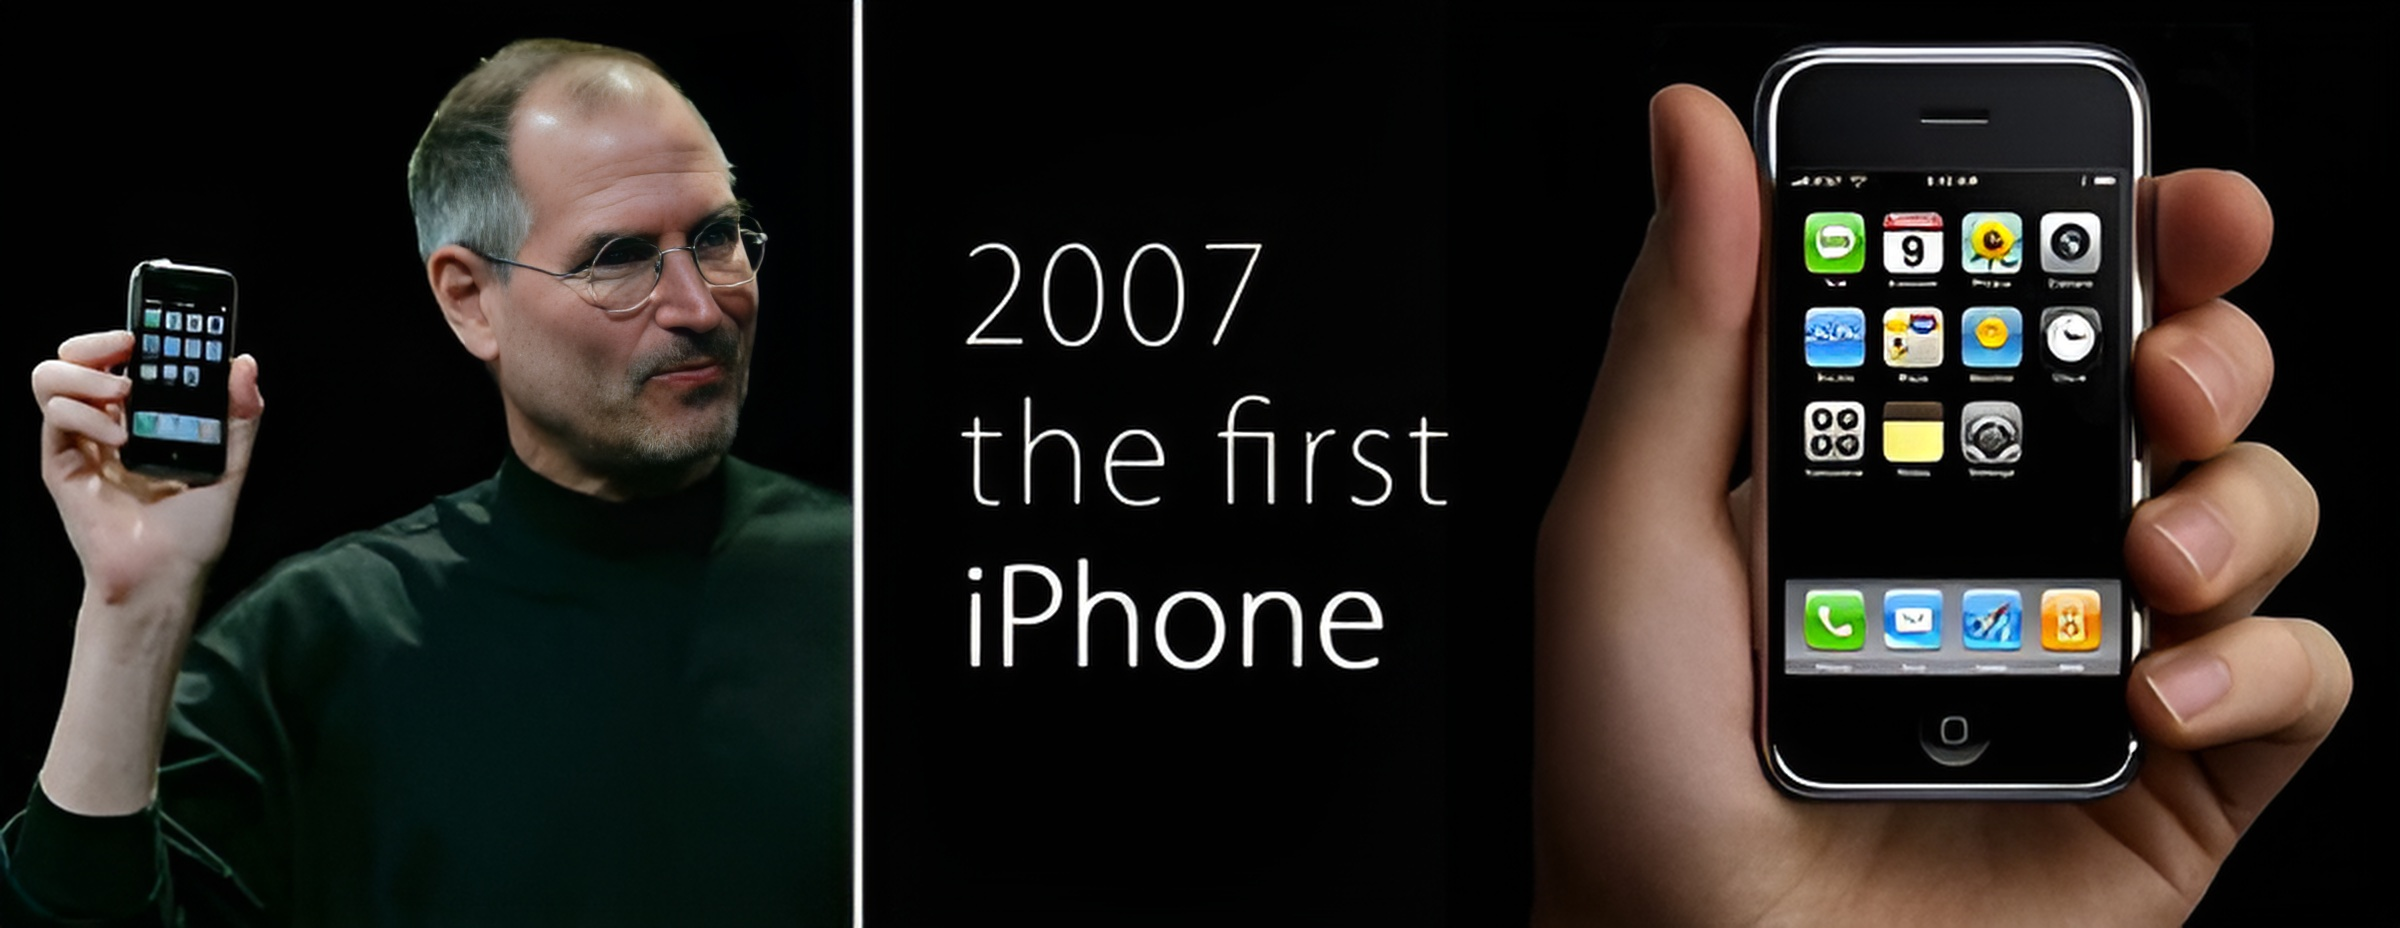
\includegraphics[width=\linewidth]{images/iphone}
    \end{figure}
\end{frame}

\begin{frame}
    \frametitle{我到哪了？}
        \begin{minipage}{0.43\linewidth}
            \begin{figure}[htpb]
                \centering
                {\bfseries 二十年前：地图}

                ~~~

                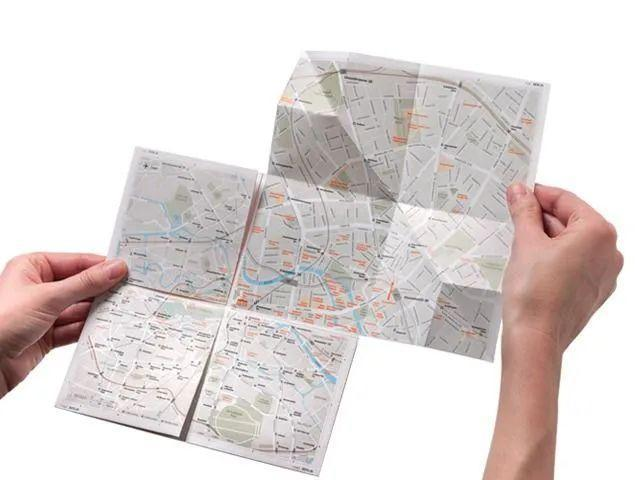
\includegraphics[height=120pt]{images/纸质地图}
            \end{figure}
        \end{minipage}\hfill
        \begin{minipage}{0.55\linewidth}
            \begin{figure}[htpb]
                \centering
                {\bfseries 现在：导航}

                ~~~

                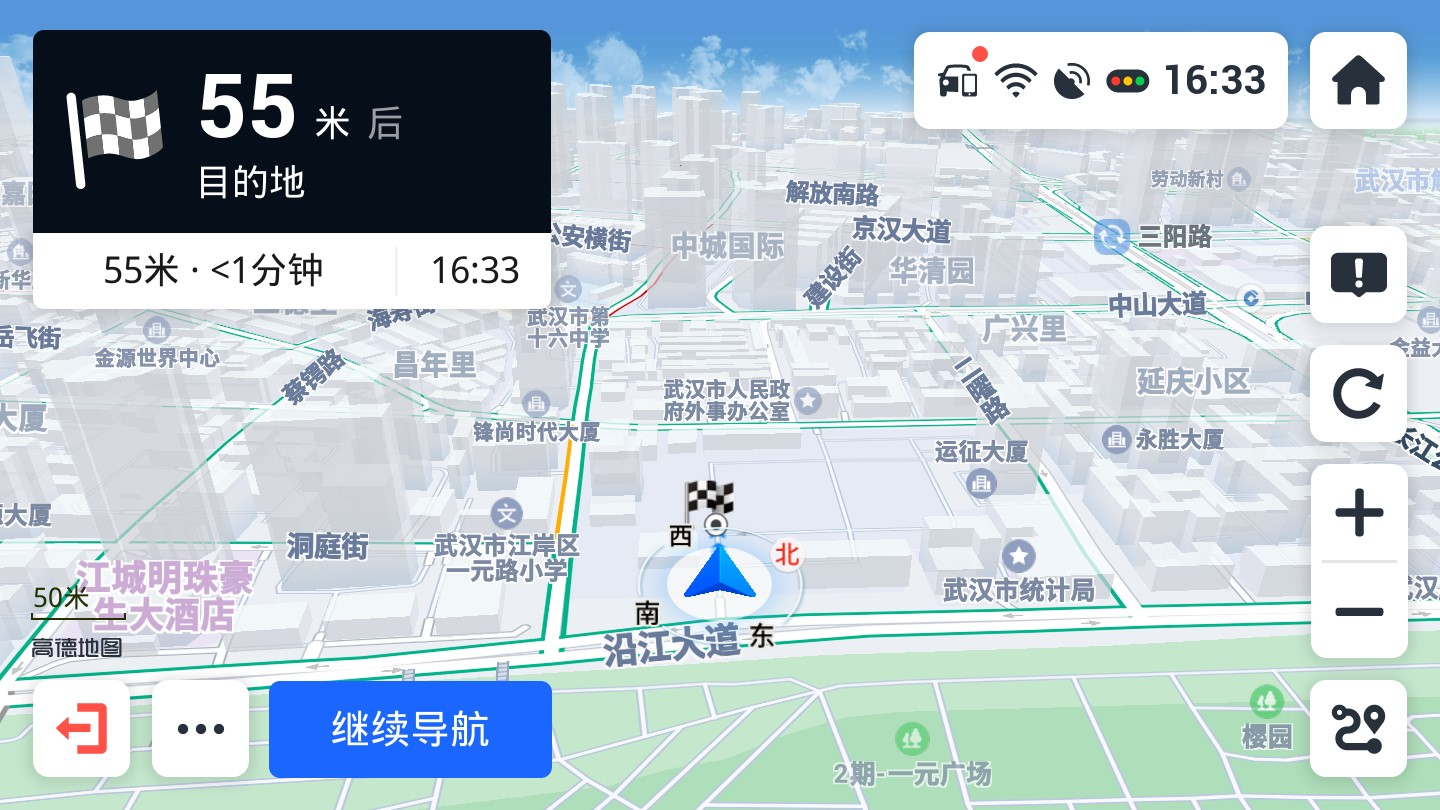
\includegraphics[height=120pt]{images/车载导航}
            \end{figure}
        \end{minipage}
\end{frame}


\begin{frame}
    \frametitle{“你在哪里？”}
        \begin{minipage}{0.48\linewidth}
            \begin{figure}[htpb]
                \centering
                {\bfseries 二十年前：“我在村口的大树下”}
                \bigskip

                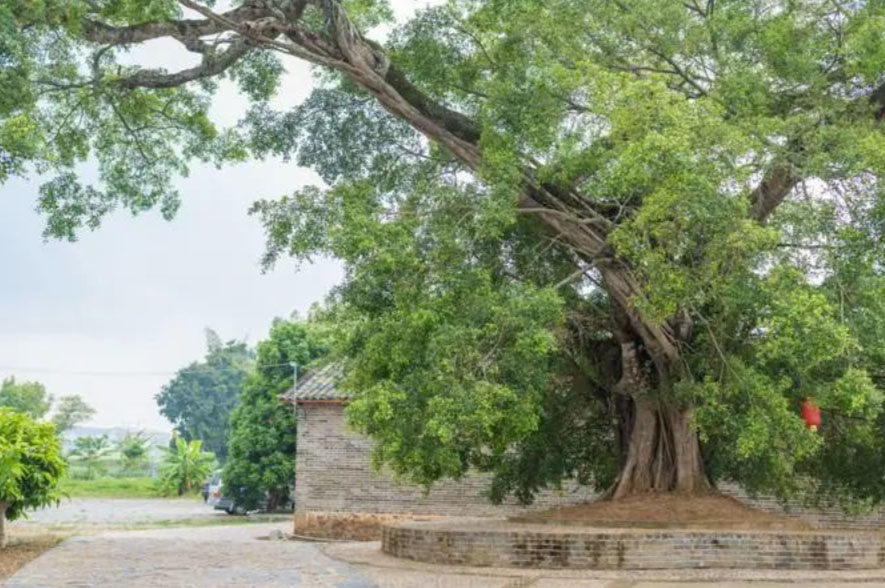
\includegraphics[height=115pt]{images/大树}
            \end{figure}
        \end{minipage}\hfill
        \begin{minipage}{0.5\linewidth}
            \begin{figure}[htpb]
                \centering
                {\bfseries 现在：卫星定位}
                \bigskip

                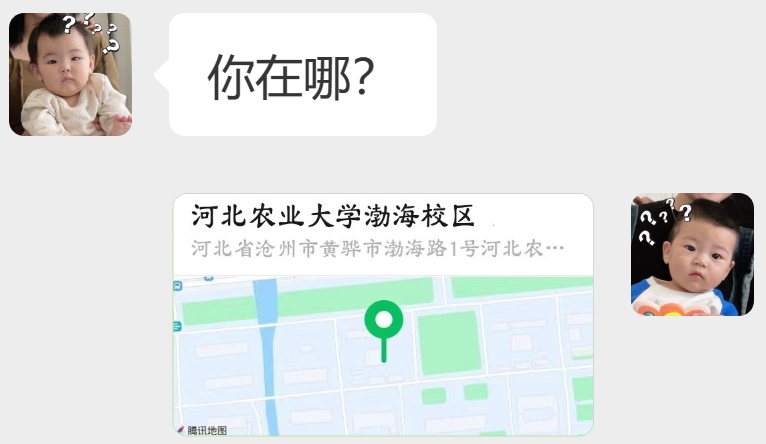
\includegraphics[height=115pt]{images/位置}
            \end{figure}
        \end{minipage}
\end{frame}



\begin{frame}
    \frametitle{海湾战争---卫星导航系统第一次大规模的使用}
    伊方拥有百万雄师，5800多辆坦克，4600多辆装甲车和步兵战车，3万门火炮，不少全球军事学家一开始都预测会打成僵持战。

    然而，只有30万军队的美国联军，仅仅用了42天，便以美军146人阵亡、467人受伤，伊军则伤亡超10万人的代价，把伊拉克的百万雄师彻底打垮。这场战争一反传统作战方式，美国对伊拉克祭出了大量精确制导武器，288枚“战斧”命中率更是高达98\% ，对伊的打击如同无头苍蝇般吊打。

    这场战争，是一场非对称战争。美军对伊拉克的打击，可以说是降维打击。因为伊拉克，还停留在机械化战争的时代。而美国，已经进入信息化战争的时代。这两种战争时代的差别，就在于有没有卫星导航系统（GPS）。

\end{frame}
\begin{frame}
    \frametitle{银河号事件}
    1993年7月23日，美国以获得情报为由，指控中国“银河号”货轮向伊朗运输制造化学武器的原料，并威胁要对中国进行制裁。美国一度直接掐断了银河号的GPS信号，让其在公海航行中失去行动力。最终，银河号只能成为砧板上的鱼肉，任人宰割。

    1993年9月4日，“银河号”货轮上最后一个货箱被检查完毕，没有发现任何化学武器，“银河号”被迫中止正常航运长达33天。

    这一事件深深地警醒了中国，如果没有自主的全球导航系统，"银河号"事件绝不会是最后一次。

    1994年12月，北斗导航实验卫星系统工程获得国家批准。
\end{frame}

\begin{frame}
    \frametitle{北斗卫星导航系统 \link{http://www.beidou.gov.cn/}}
    北斗卫星导航系统（以下简称北斗系统）是中国着眼于国家安全和经济社会发展需要，自主建设运行的全球卫星导航系统，是为全球用户提供全天候、全天时、高精度的定位、导航和授时服务的国家重要时空基础设施。 
    \bigskip

    “三步走”发展历程：
        \begin{itemize}
          \item 2000年年底，建成北斗一号系统，向中国提供服务；
          \item 2012年年底，建成北斗二号系统，向亚太地区提供服务；
          \item 2020年，建成北斗三号系统，向全球提供服务。 
        \end{itemize}
\end{frame}

\begin{frame}
    \frametitle{新时代北斗精神}
    \begin{center}        
        {\huge \cbf{自主创新、开放融合、万众一心、追求卓越}} % 新时代北斗精神
    \end{center}    
\end{frame}

\begin{frame}
    \frametitle{北斗 VS GPS}
\begin{table}[]
    \begin{tabular}{@{}lll@{}}
    \toprule
    \multicolumn{1}{c}{} & \multicolumn{1}{c}{北斗} & \multicolumn{1}{c}{GPS} \\ \midrule
    卫星覆盖                 & 55颗                    & 31颗                     \\
    通讯信号                 & 三频信号                   & 双频信号                    \\
    短报文通信                & 北斗独创                   & 无                       \\
    分步开通                 & 支持局部卫星组网               & 必须全部卫星                  \\
    民用定位精度 \qquad              & 10米，亚太地区5m    \qquad         & 10米                     \\
    军用定位准度               & 0.5米                   & 0.3米                    \\ \bottomrule
    \end{tabular}
    \end{table}
\end{frame}


\begin{frame}
    \frametitle{华为Mate50，短报文通信\link{http://www.beidou.gov.cn/yw/xwzx/202209/t20220929_24645.html}}
    \begin{figure}[htpb]
        \centering
        \setcounter{subfigure}{0}
        \subfloat{
\includegraphics[height=6cm]{mate50}}\hfill
        \subfloat{
\includegraphics[height=6cm]{mate50-2}}
    \end{figure}
\end{frame}


\begin{frame}
    \frametitle{华为Mate60，卫星电话}
    \begin{figure}[htpb]
        \centering
        
\includegraphics[width=.8\linewidth]{mate60}
    \end{figure}
\end{frame}


\begin{frame}
    \frametitle{天通一号卫星移动通信系统\link{http://www.tdstar.cn/industry/157.html}}

    \begin{itemize}
      \item 01星2016年发射，中国地区无缝覆盖（领土/领海/第一岛链）
      \item 02/03星覆盖亚洲17个国家：日本、韩国、菲律宾、帕劳、越南、老挝、柬埔寨、泰国、马来西亚、新加坡、印尼、文莱、东帝汶、缅甸、孟加拉国、不丹、尼泊尔
    \end{itemize}
    \begin{figure}[htpb]
        \centering
        
\includegraphics[width=.7\linewidth]{天通}
    \end{figure}
\end{frame}


% 北斗的未来，是大众规模化应用。因为卫星导航系统非常烧钱，无论是早期的研发，发射卫星，还是后期的维护运营，都非常烧钱。卫星也是有使用寿命的，报废了就得再发射一颗上去。所以北斗也要恰饭，要挣钱养活自己才行。美国的GPS是怎么挣钱养活自己的呢？它是通过卖GPS定位芯片，来挣钱的。咱们每个人手机里，都有美国GPS的定位芯片，每一个芯片，都需要向美国人交授权费才能用。2017年以后，随着国产手机的强势崛起，华为、小米、OPPO等品牌在世界手机行业站稳脚跟，北斗也找到了自己的用武之地。这两三年你买的国产手机里，都安装有北斗系统，都有北斗芯片，你已经用真金白银，为北斗助力了。

% 北斗系统未来在全球应用市场的基本格局：

% 第一，北斗在全球最大的应用市场，肯定是在中国。

% 虽然目前美国GPS占据了中国很大的民用市场，但未来北斗系统肯定会逐渐取而代之，美国GPS在中国将逐渐变成北斗的辅助系统，而非主流的卫星导航系统。

% 第二，北斗在全球最难抢占的市场，肯定是美国、欧洲、俄罗斯、印度、日本这些拥有自主卫星导航系统的国家，甚至很难抢占加拿大、澳大利亚等亲美国家的主流市场。

% 很难抢占主流市场，并不意味着无法进入，毕竟北斗系统拥有一些独特的技术优势，如果GPS、伽利略、格洛纳斯等系统可以和北斗系统兼容使用，就能提供更加稳定、更高精度的授时、定位和导航服务。另外，目前只有北斗可以提供短报文服务，这一功能在地面通讯不畅时，能够发挥关键的作用，美国也在使用北斗的短报文服务。

% 所以，寻求合作共赢，这就是中国北斗能够进入欧美俄罗斯市场的基本逻辑。目前北斗已经实现和GPS、格洛纳斯系统的兼容，还在进一步推动与其他系统的兼容。

% 第三，北斗在全球竞争最激烈的市场，是那些没有自主卫星导航技术的国家，包括非洲、南美、南亚、中亚、西亚等。

% 这部分市场空间非常大，美国GPS已经深耕二十多年，中国北斗要想进入，必然要与美国GPS短兵相接。其实，这些没有自主卫星导航技术的国家，更担心本国的军事安全，虽然可以免费使用美国GPS，但也担心美国老大哥随时关闭或者故意扰乱卫星信号。

% 但这些国家没钱、也没技术发射导航卫星，又能怎么办？

% 最佳的策略就是同时使用不同的全球卫星导航技术，既确保不受制于某一个国家，又可以引入竞争，获得精度更高、运行更稳定的服务。

% 充分竞争，这就是中国北斗可以快速进入亚非拉国家的基本逻辑。

% 目前北斗二代的相关产品已经逐步输出到100多个国家，北斗三代的产品将会利用一带一路等政策优势，以更大的步伐走向亚非拉国家的每一个角落，促进北斗产品和服务的普及。

\begin{frame}
    \frametitle{卫星导航主要应用场景}
    \begin{itemize}
      \item {\cbf{地理数据采集}} \quad 国土、矿产和环境调查；铁路、公路、电力、水利等位置信息
      \item {\cbf{高精度测量}} \qquad 大地测量、资源勘查、地壳运动、工程测量、海洋测量
      \item {\cbf{车辆监控调度}} \quad 对车辆进行调度和管理
      \item {\cbf{航空和航海}} \qquad 空中交通管理系统、导航救援、港口运作
      \item {\cbf{军用}} \qquad \qquad \quad 导航定位、精确制导
      \item {\cbf{时间和同步}} \qquad 通信网络、电力网络授时与时间同步
      \item {\cbf{机械控制}} \qquad \quad 农业机械、工业机械、无人机控制
      \item {\cbf{消费应用}} \qquad \quad 手机导航、车载导航、通信应用
    \end{itemize}
\end{frame}

\begin{frame}
    \frametitle{GNSS技术在农业中的应用}
    \begin{itemize}
        \item {\cbf{农田测绘}}
        
        过去，农田测绘依赖的是用双脚丈量土地。测绘人员沿着农田的边界行走，通过携带的 GPS 手持测绘器采集边界的经纬坐标，通过采集得到的边界数据获取农田面积、地理位置等数据信息。现在，测绘无人机取代了测绘人员一步一脚印的采集方式，效率更高、速度更快，更是大大降低了采集过程的劳动强度。
        \item {\cbf{智能农机导航}}
        
        在耕种、收割、施肥、喷药的农业机械上安装车载GPS定位器，能程序化地跟从已定的路线进行耕种施肥或者进行农药喷洒，合理化的路线有效减少了肥料和农药的使用。
        \item {\cbf{精准喷药 }}
        
        DGPS航空导航系统可以引导飞行员从机场直接前往作业区，在已设计的航线和高度飞行喷洒药物，若加满药物再次返回作业区时，还能让飞机到达上次药物喷洒停止时的准确地点，以确保既无重复喷洒又无遗漏区域。
      \end{itemize}
\end{frame}

\begin{frame}
    \frametitle{遥感技术 RS}
    遥感一词来源于英语“Remote Sensing”，其直译为“遥远的感知”，时间长了人们将它简译为“遥感”。
    
    遥感是指运用现代光学、电子学探测仪器，不与目标物相接触，从远距离把目标物的电磁波特性记录下来，通过分析，揭示出物体的特征性质及其变化的综合性探测技术。

    \begin{figure}[htpb]
        \centering
        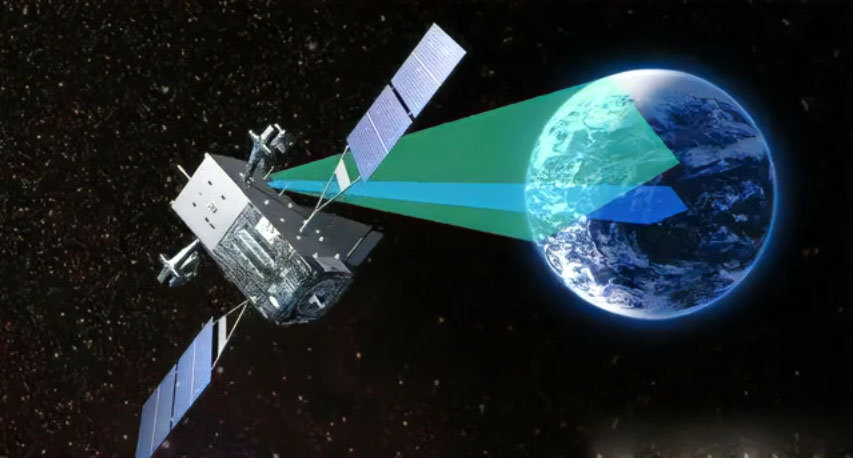
\includegraphics[height=.26\linewidth]{images/遥感1}
        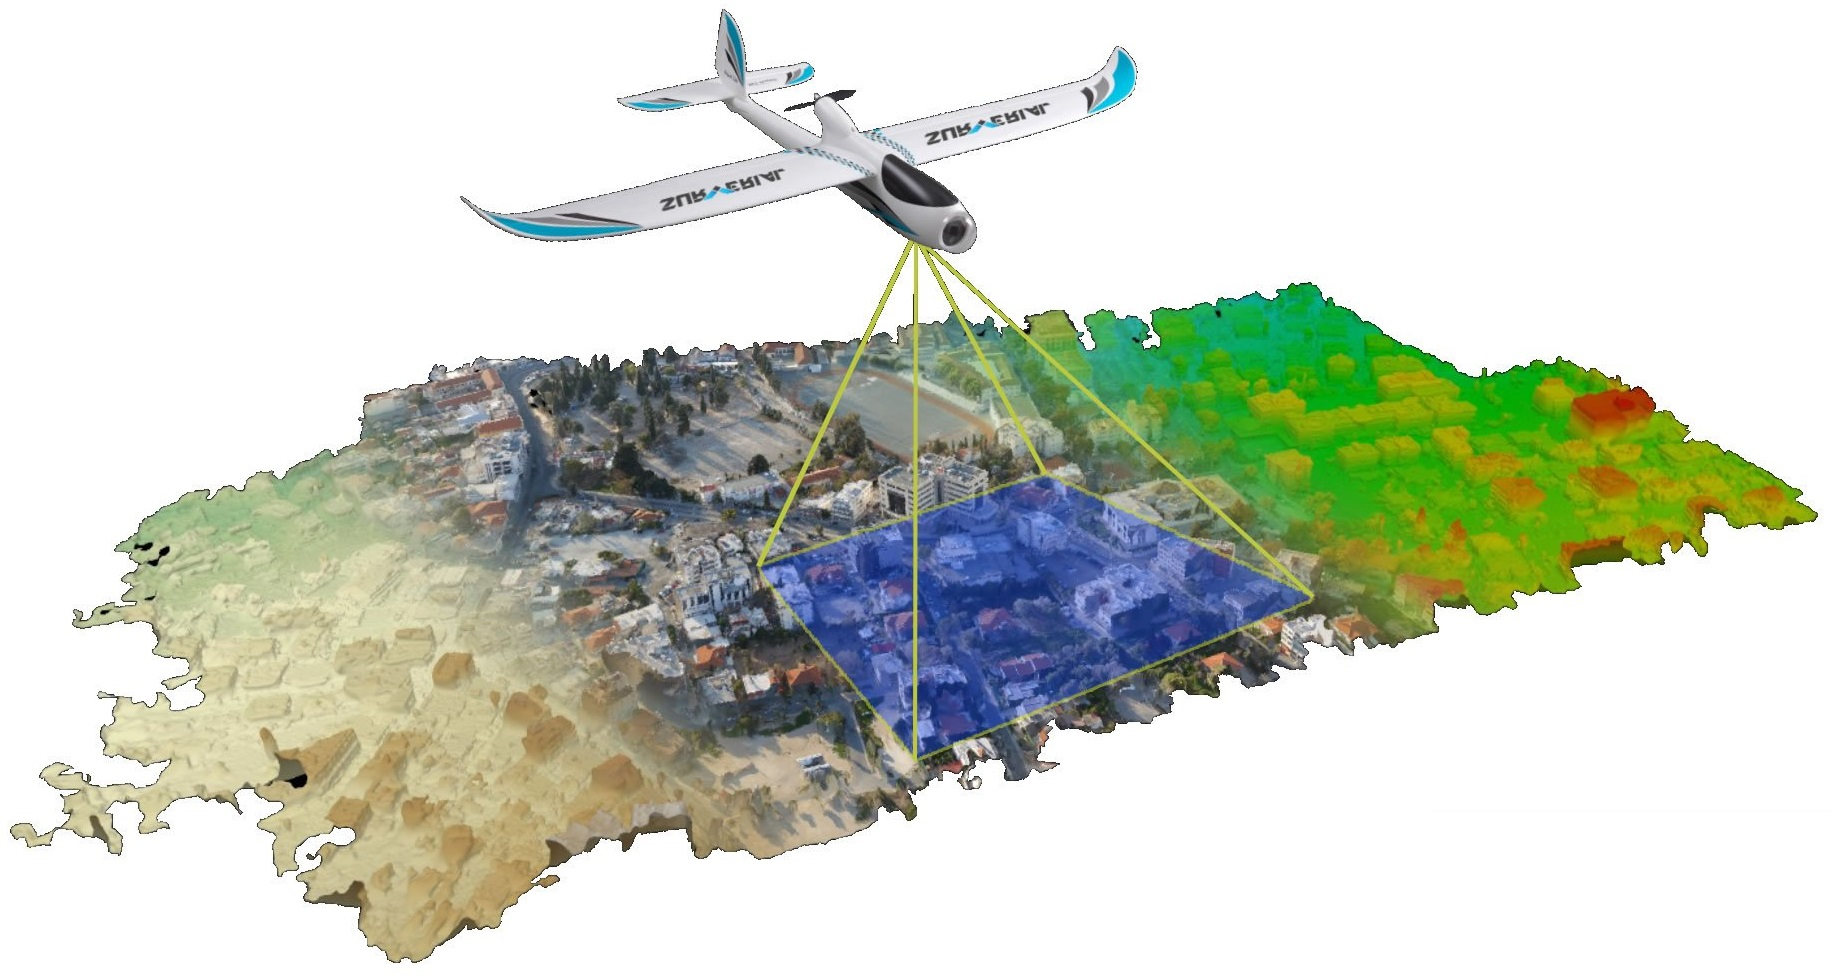
\includegraphics[height=.26\linewidth]{images/遥感2}
    \end{figure}

\end{frame}

\begin{frame}
    \frametitle{遥感技术原理}
    \begin{figure}[htpb]
        \centering
        {\bfseries 不同地物对电磁波辐射、反射、吸收的特性不同 \qquad}
        \smallskip

        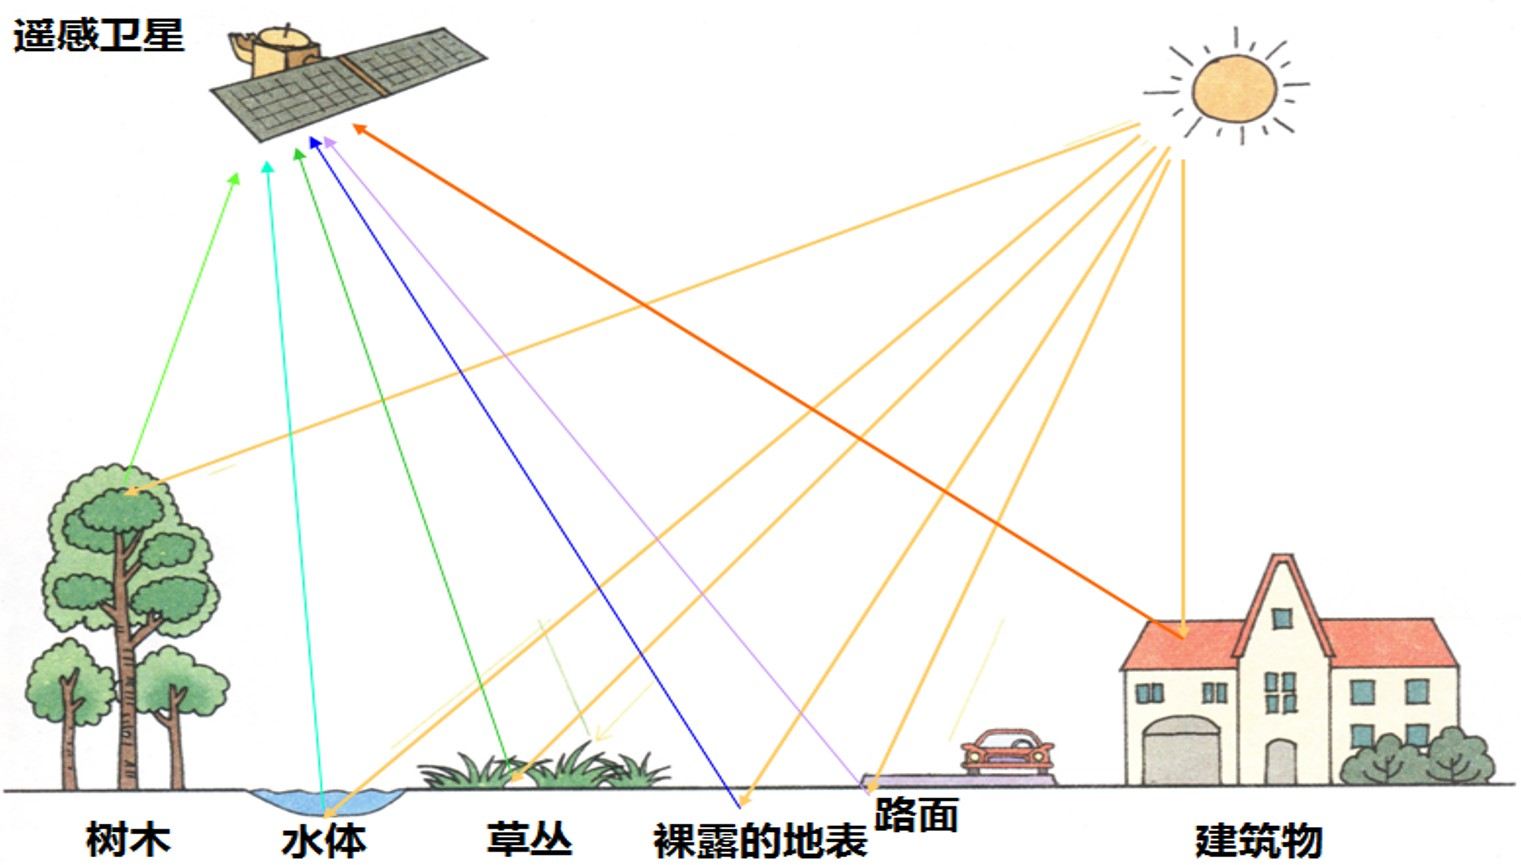
\includegraphics[height=.4\linewidth]{images/遥感原理}
    \end{figure}
\end{frame}
%  遥感之所以能苟根据收集到的电磁波信息来识别地物目标，是因为有信息源的存在。信息源是遥感探测的依据，任何物体都具有发射、反射和吸收电磁波的特性，目标地物与电磁波之间的相互作用构成物体的电磁波特性。因此，遥感技术主要是建立在物体辐射和反射电磁波的原理之上。目标物体的电磁波特性由传感器来获取，通过返回舱或微波天线传至地面接受站。地面接收站将接收到的信息进行存储和处理，转换成用户可以使用的各种数据格式。用户再按照不同的应用目的对这些信息进行分析处理，以达到遥感应用的目的。

\begin{frame}
    \frametitle{遥感系统组成}
    \begin{figure}[htpb]
        \centering
        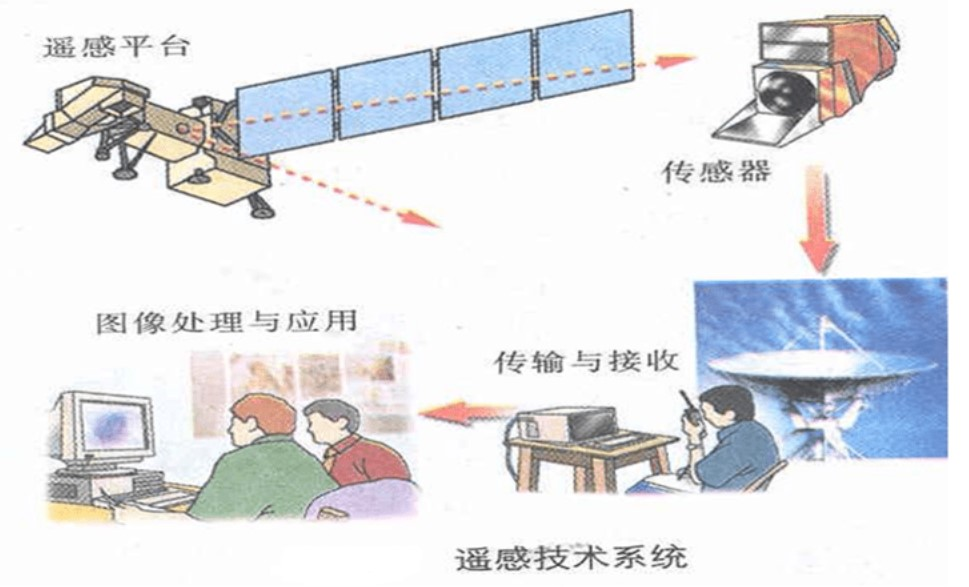
\includegraphics[height=.44\linewidth]{images/遥感组成}
    \end{figure}
\end{frame}

\begin{frame}
    \frametitle{遥感图像}
    \begin{figure}[htpb]
        \centering
        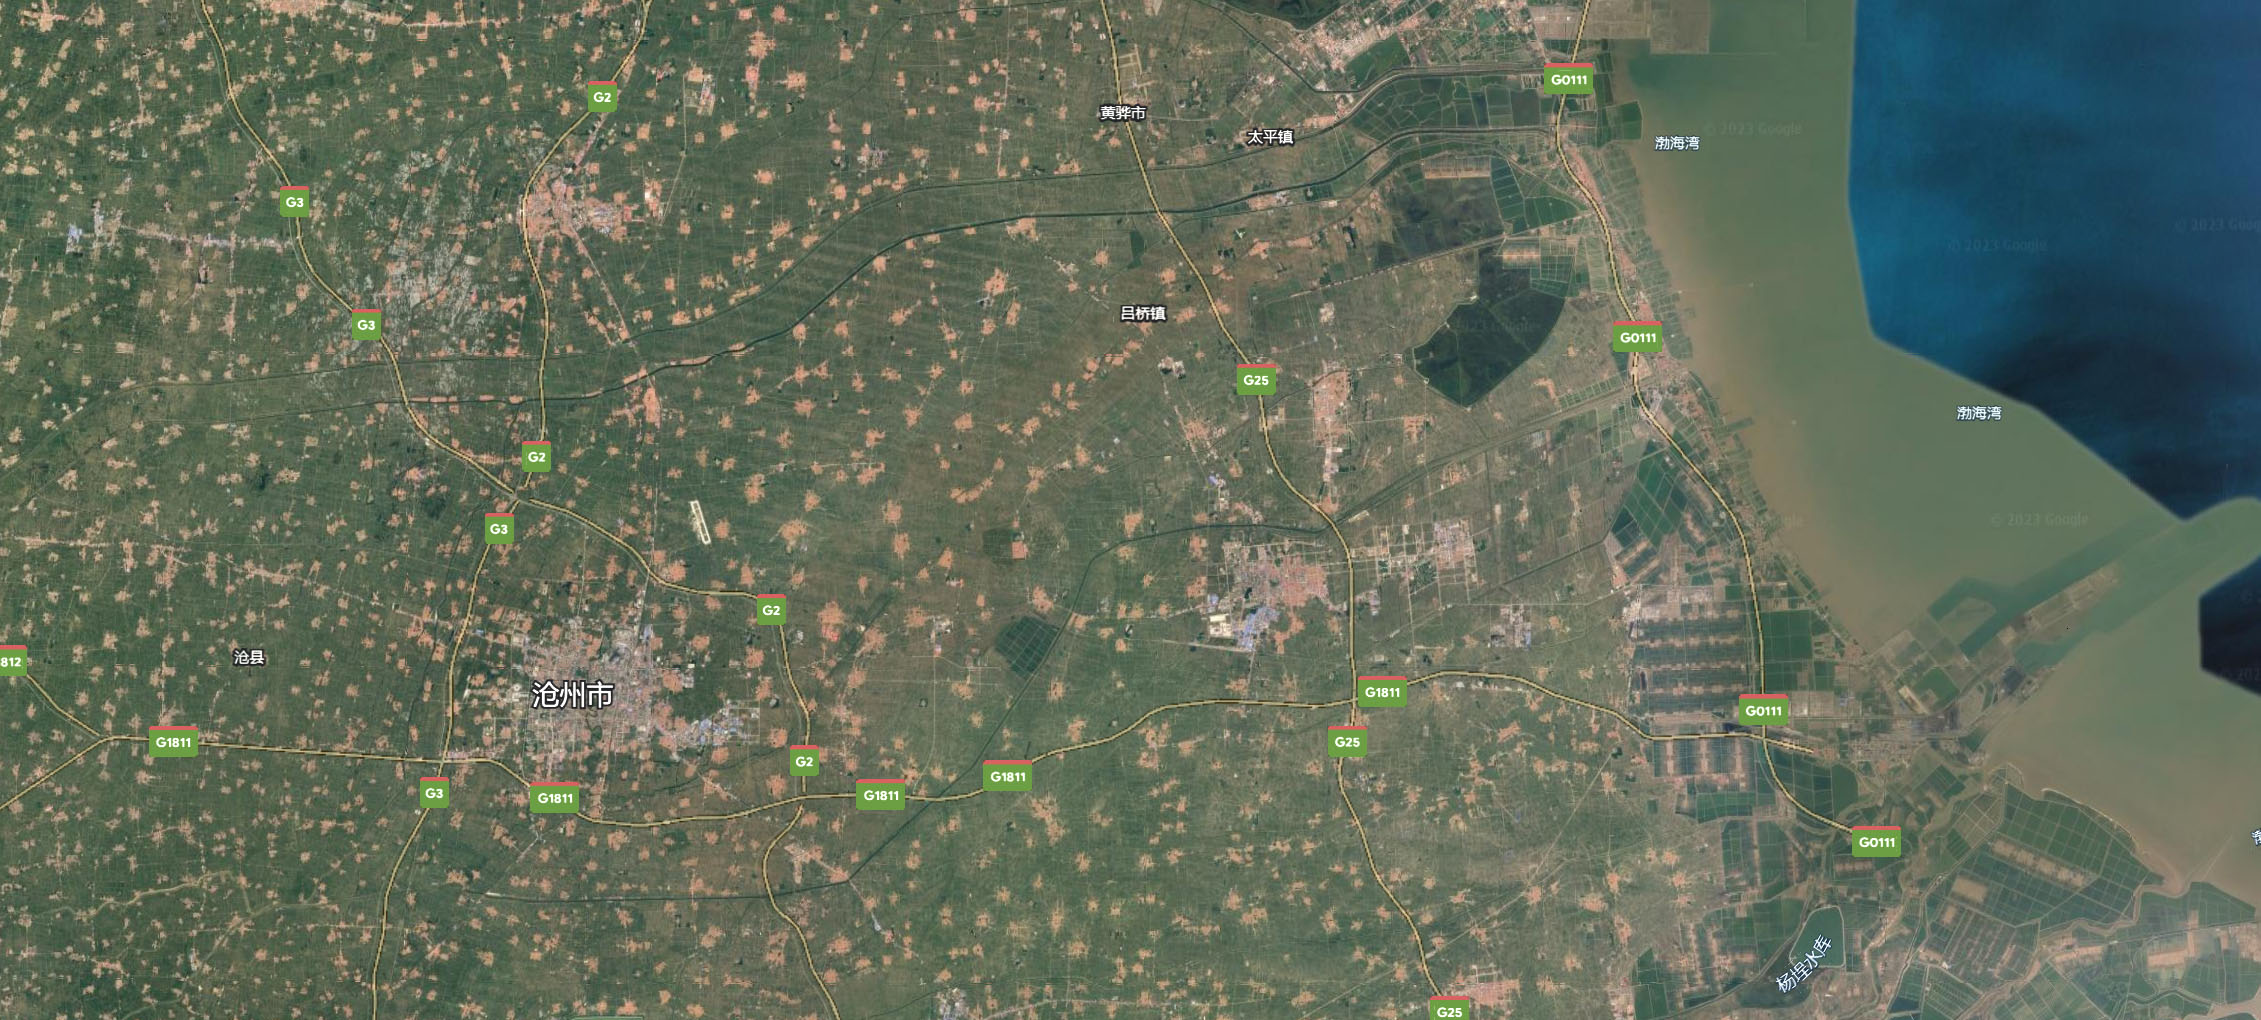
\includegraphics[height=.44\linewidth]{images/遥感图像2}
    \end{figure}
\end{frame}

\begin{frame}
    \frametitle{遥感图像}
    \begin{figure}[htpb]
        \centering
        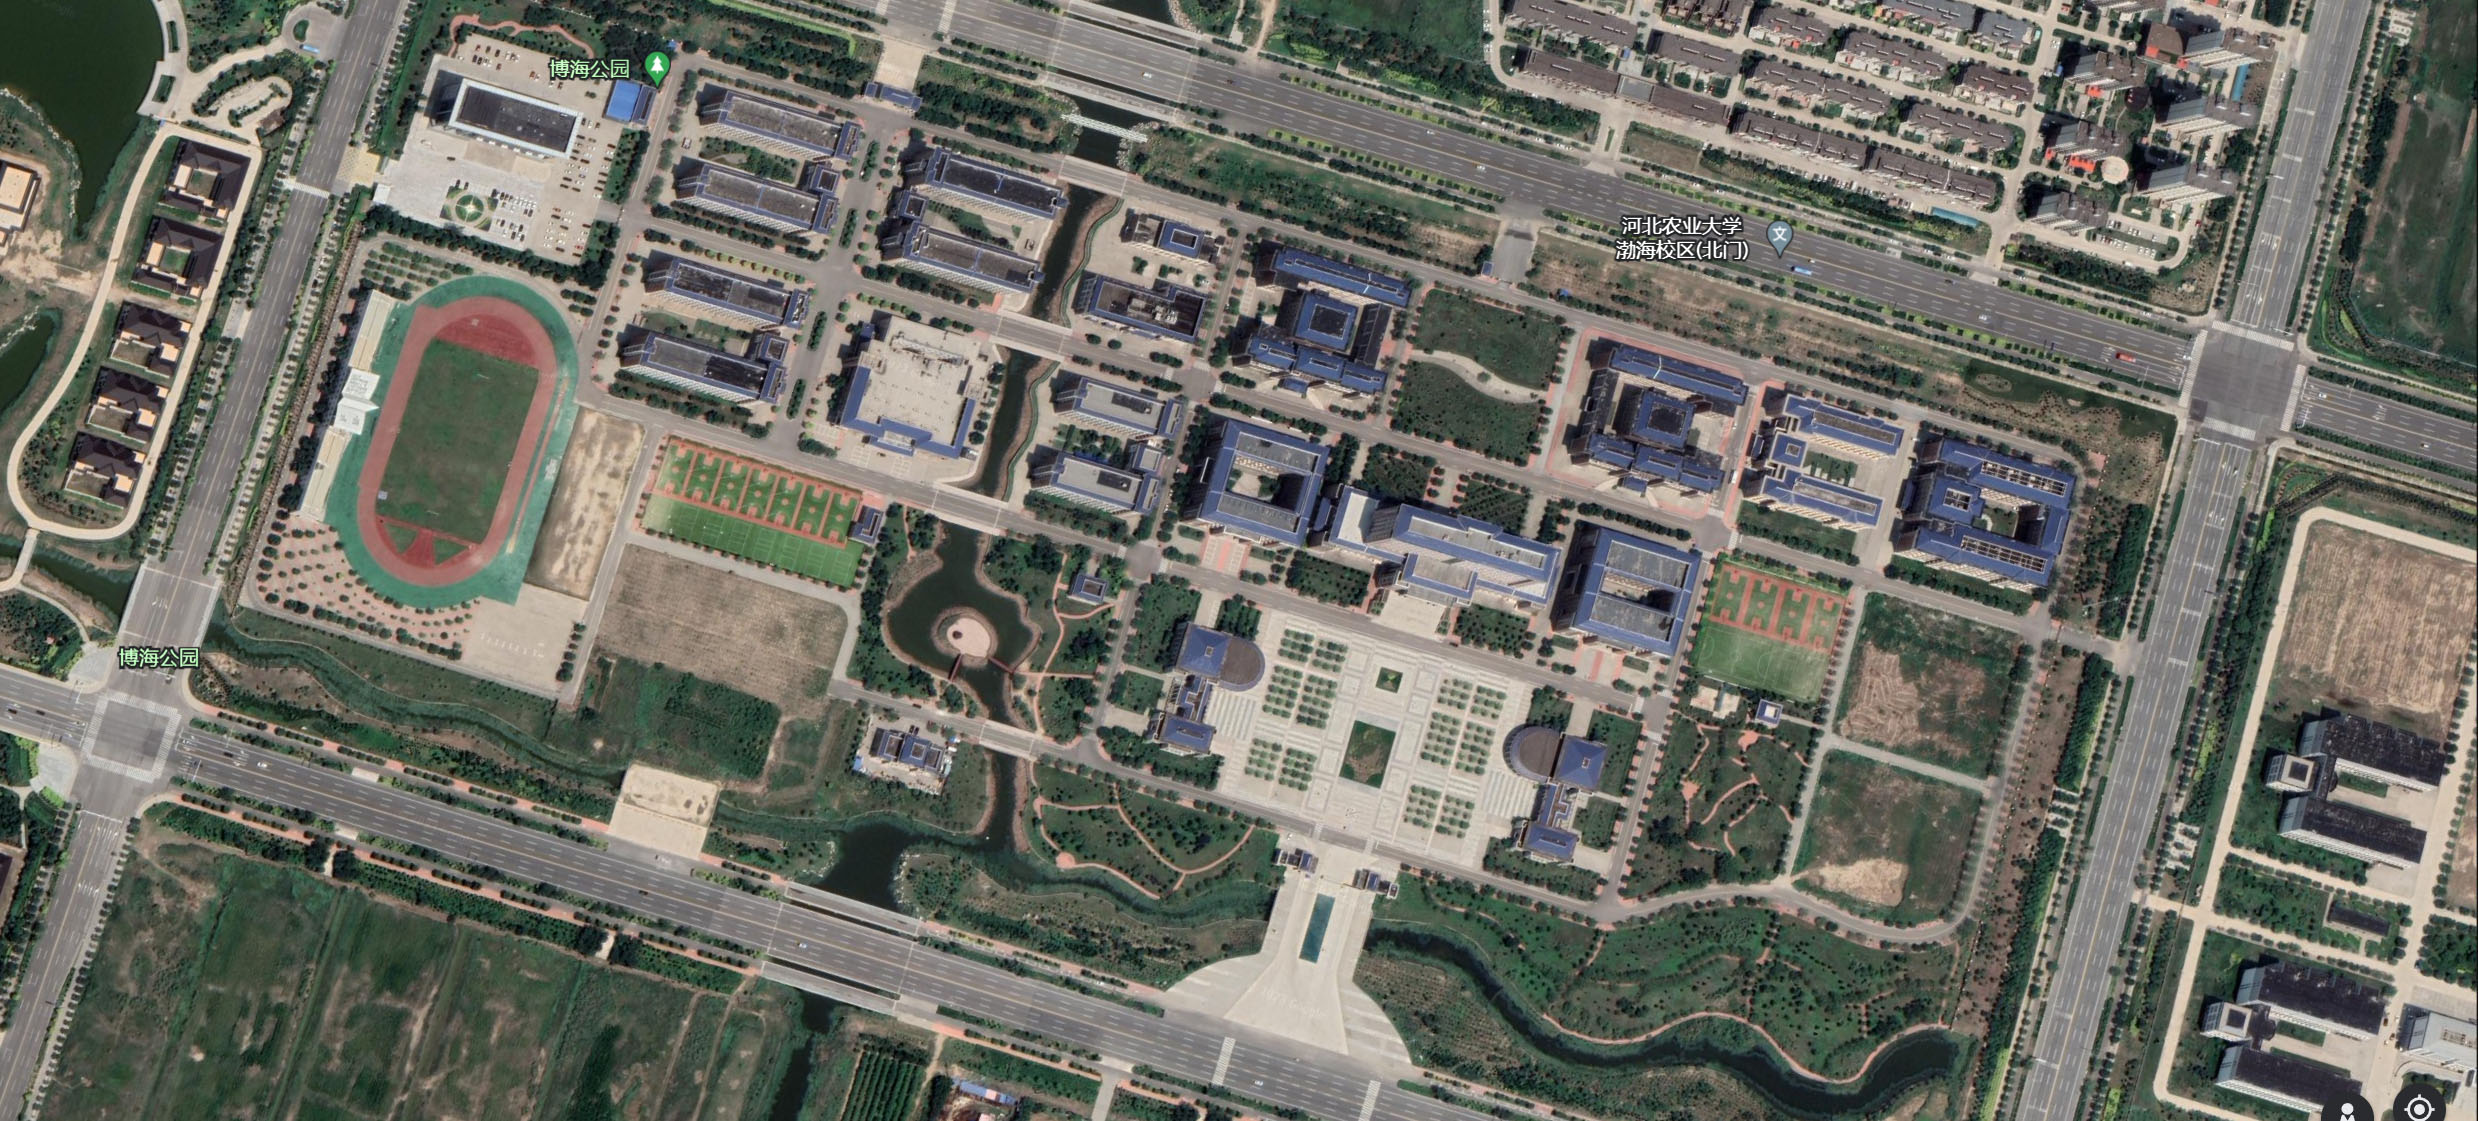
\includegraphics[height=.44\linewidth]{images/遥感图像}
    \end{figure}
\end{frame}


\begin{frame}
    \frametitle{遥感的分类}
    按遥感平台的高度分类大体上可分为航天遥感、航空遥感和地面遥感。
    \Large{
        \begin{itemize}
            \item {\cbf{天}} \qquad \faSatellite \quad \faIcon{space-shuttle} \quad \faIcon{rocket}
            
            \item {\cbf{空}} \qquad \faIcon{plane} \quad \faIcon{helicopter} \quad \faIcon{parachute-box} 
            \item {\cbf{地}} \qquad \faIcon{truck-monster} \quad \faIcon{ship} \quad \faIcon{archway}
            
            \item {\cbf{其它}} \quad \faIcon{internet-explorer} \quad\faIcon{people-arrows} 
        \end{itemize}}
\end{frame}


\begin{frame}
    \frametitle{天宫空间站}
    \begin{figure}[htpb]
        \centering
        
\includegraphics[width=.8\linewidth]{空间站}
    \end{figure}
    \vspace{-4pt}
\end{frame}


\begin{frame}
    \frametitle{天宫空间站}
    \newcommand{\foo}{\color{maincolor}\makebox[0pt]{\textbullet}\hskip-0.5pt\vrule width 1pt\hspace{\labelsep}}
    \begin{table}
        \centering
        \renewcommand\arraystretch{1.4}\arrayrulecolor{maincolor}
        \begin{tabular}{@{\,}r <{\hskip 2pt} !{\foo} >{\raggedright\arraybackslash}p{.8\linewidth}}
        2010.9 & 中央专门委员会批准实施载人空间站工程 \\
        2012.3 & 天宫空间站完成了立项综合论证转入方案设计阶段 \\
        2014.6 & 天宫空间站结束方案设计阶段工作转入初样研制阶段 \\
        2021.4 & 天和核心舱发射 \\
        2021.6 & 神舟十二号发射，聂海胜、刘伯明、汤洪波首批入驻中国空间站\\
        2022.7 & 问天实验舱发射 \\
        2022.10 & 梦天实验舱发射 \\
        2022.12 & 中国国家主席习近平在新年贺词中宣布，“中国空间站全面建成” \\
        \end{tabular}
    \end{table}
\end{frame}


\begin{frame}
    \frametitle{2024年6月，嫦娥六号任务取得圆满成功}
    \begin{figure}[htpb]
        \centering
        
\includegraphics[width=.9\linewidth]{嫦娥六号}
    \end{figure}
\end{frame}


\begin{frame}
    \frametitle{各国探月计划}
    \vspace{-0.5em}
    \begin{figure}[htpb]
        \centering
        \setcounter{subfigure}{0}
        \subfloat[中国探月计划]{
\includegraphics[height=6.5cm]{中国探月}}\quad
        \subfloat[世界各国探月计划]{
\includegraphics[height=6.5cm]{世界探月}}
    \end{figure}
\end{frame}


\begin{frame}
    \frametitle{中国探月工程}
    \newcommand{\foo}{\color{maincolor}\makebox[0pt]{\textbullet}\hskip-0.5pt\vrule width 1pt\hspace{\labelsep}}
    \begin{table}
        \centering
        \renewcommand\arraystretch{1.4}\arrayrulecolor{maincolor}
        \begin{tabular}{@{\,}r <{\hskip 2pt} !{\foo} >{\raggedright\arraybackslash}p{.8\linewidth}}
        2004 & 中国正式开展月球探测工程 \\
        2007.10 & 嫦娥一号成功发射 \\
        2010.10 & 嫦娥二号发射 \\
        2013.12 & 嫦娥三号着陆月面\\
        2018.12 & 嫦娥四号，人类第一个着陆月球背面的探测器 \\
        2020.12 & 嫦娥五号返回器携带月球样品返回地球 \\
        2024.6 & 嫦娥六号采集月球背面样品1935.3克 \\
        \end{tabular}
    \end{table}
\end{frame}


\begin{frame}
    \frametitle{遥感的分类}
    \begin{itemize}
      \item 按所利用的电磁波的光谱段分类：
        \begin{itemize}
            \item 可见反射红外遥感
            \item 热红外遥感
            \item 微波遥感
        \end{itemize}
      \item 按研究对象分类：
        \begin{itemize}
            \item 资源遥感
            \item 环境遥感
        \end{itemize}
      \item 按应用空间尺度分类：
        \begin{itemize}
            \item 全球遥感
            \item 区域遥感
            \item 城市遥感
        \end{itemize}    
    \end{itemize}
\end{frame}


\begin{frame}
    \frametitle{无人机遥感及其优势}
    以无人机为平台，负载数码相机、数码摄录机等数字遥感设备进行拍摄和记录，通过数据处理技术进行影像的同步传输，实现对地理信息的实时调查与监测。
    \begin{enumerate}
      \item 响应能力快：无人机的低空飞行便于空域申请，同时也降低了对天气条件的要求。升空准备时间短、操作相对简单。
      \item 图像分辨率高：无人机遥感可获取到超高分辨率数字影像和定位数据，可针对特殊监测目标搭载全色波段、单波段、多波段等传感器，也可以进行多角度摄影。
      \item 应用拓展能力强：系统为多种小型遥感传感器提供了多个搭载平台，如探地雷达、热成像仪、SAR等，便于扩展监测功能。
      \item 运营成本低：系统的置建费成本较低，运营成本、维护成本和操作人员的成本要低于载人机系统。
    \end{enumerate}

\end{frame}


\begin{frame}
    \frametitle{大疆---无人机市场引领者\link{https://www.dji.com/cn}}
    \begin{figure}[htpb]
        \centering
        \setcounter{subfigure}{0}
        \subfloat[消费级]{
\includegraphics[height=4cm]{消费级}}\hfill
        \subfloat[专业级]{
\includegraphics[height=4cm]{专业级}}\hfill
        \subfloat[农业无人机]{
\includegraphics[height=4cm]{农业}}
    \end{figure}
\end{frame}

\begin{frame}
    \frametitle{遥感技术在农业中的应用}
    \begin{enumerate}
      \item {\cbf{作物种植面积与长势监测}}
      
      由于不同的作物在遥感影像上呈现不同的颜色、纹理、形状等特征信息，运用卫星与无人机遥感技术获取的遥感影像，利用信息提取的方法，提取作物的种植区域，可快速、大面积获得田间作物种植面积与分布数据。此外，遥感影像还可以实时记录作物不同阶段的生长状况，获得同一地点时间序列的图像了解不同生育阶段的作物长势。% 传统的人工测量，耗时长，效率低。田间调查取样一个小时，只能完成200亩左右。
      \item {\cbf{作物病虫害监测}}
      
      植被对诸如病虫害、肥料缺乏等胁迫的反应随胁迫的类型和程度的不同而变化，相应的，植物特征吸收曲线特别是红色区和红外区的光谱特性就会发生相应变化，所以在病害早期就可通过遥感探测到。% https://zhuanlan.zhihu.com/p/269850549
      \item {\cbf{作物遥感估产 \link{http://www.gov.cn/xinwen/2022-12/12/content_5731454.htm}}}
      
      利用现场测产与遥感卫星数据，建立遥感测产模型，就可以完成对作物的估产，估产结果准确率通常在90\%以上。
    \end{enumerate}
\end{frame}

\begin{frame}
    \frametitle{地理信息系统 GIS}
    地理信息系统（Geographic Information System）是一种特定的十分重要的空间信息系统。它是在计算机硬、软件系统支持下，对整个或部分地球表层（包括大气层）空间中的有关地理分布数据进行采集、储存、管理、运算、分析、显示和描述的技术系统。

    GIS技术把地图这种独特的视觉化效果和地理分析功能与一般的数据库操作集成在一起。

\end{frame}

\begin{frame}
    \frametitle{国家地理信息公共服务平台 \link{https://www.tianditu.gov.cn/}}
    \begin{figure}[htpb]
        \centering
        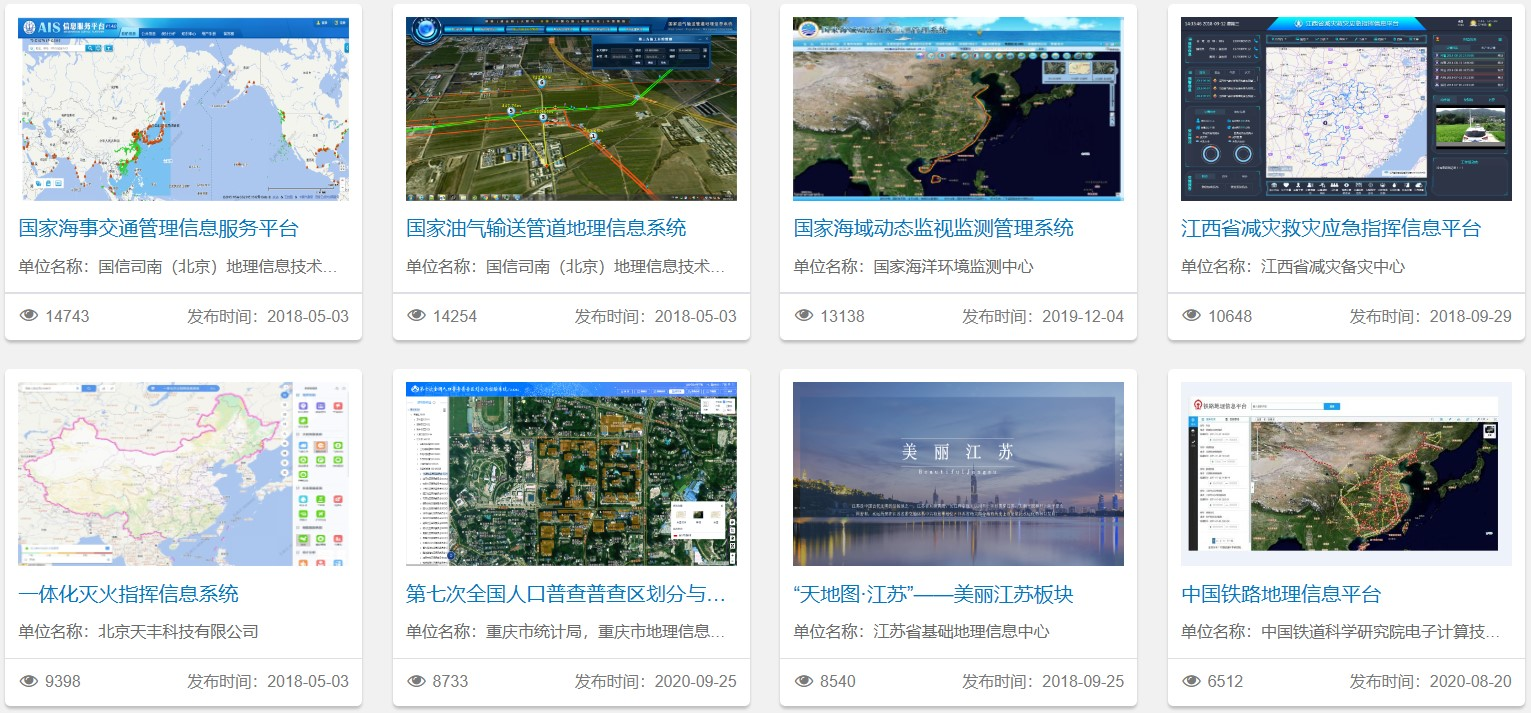
\includegraphics[height=.44\linewidth]{images/天地图}
    \end{figure}
\end{frame}

\begin{frame}
    \frametitle{粮食产量}
    \begin{figure}[htpb]
        \centering
        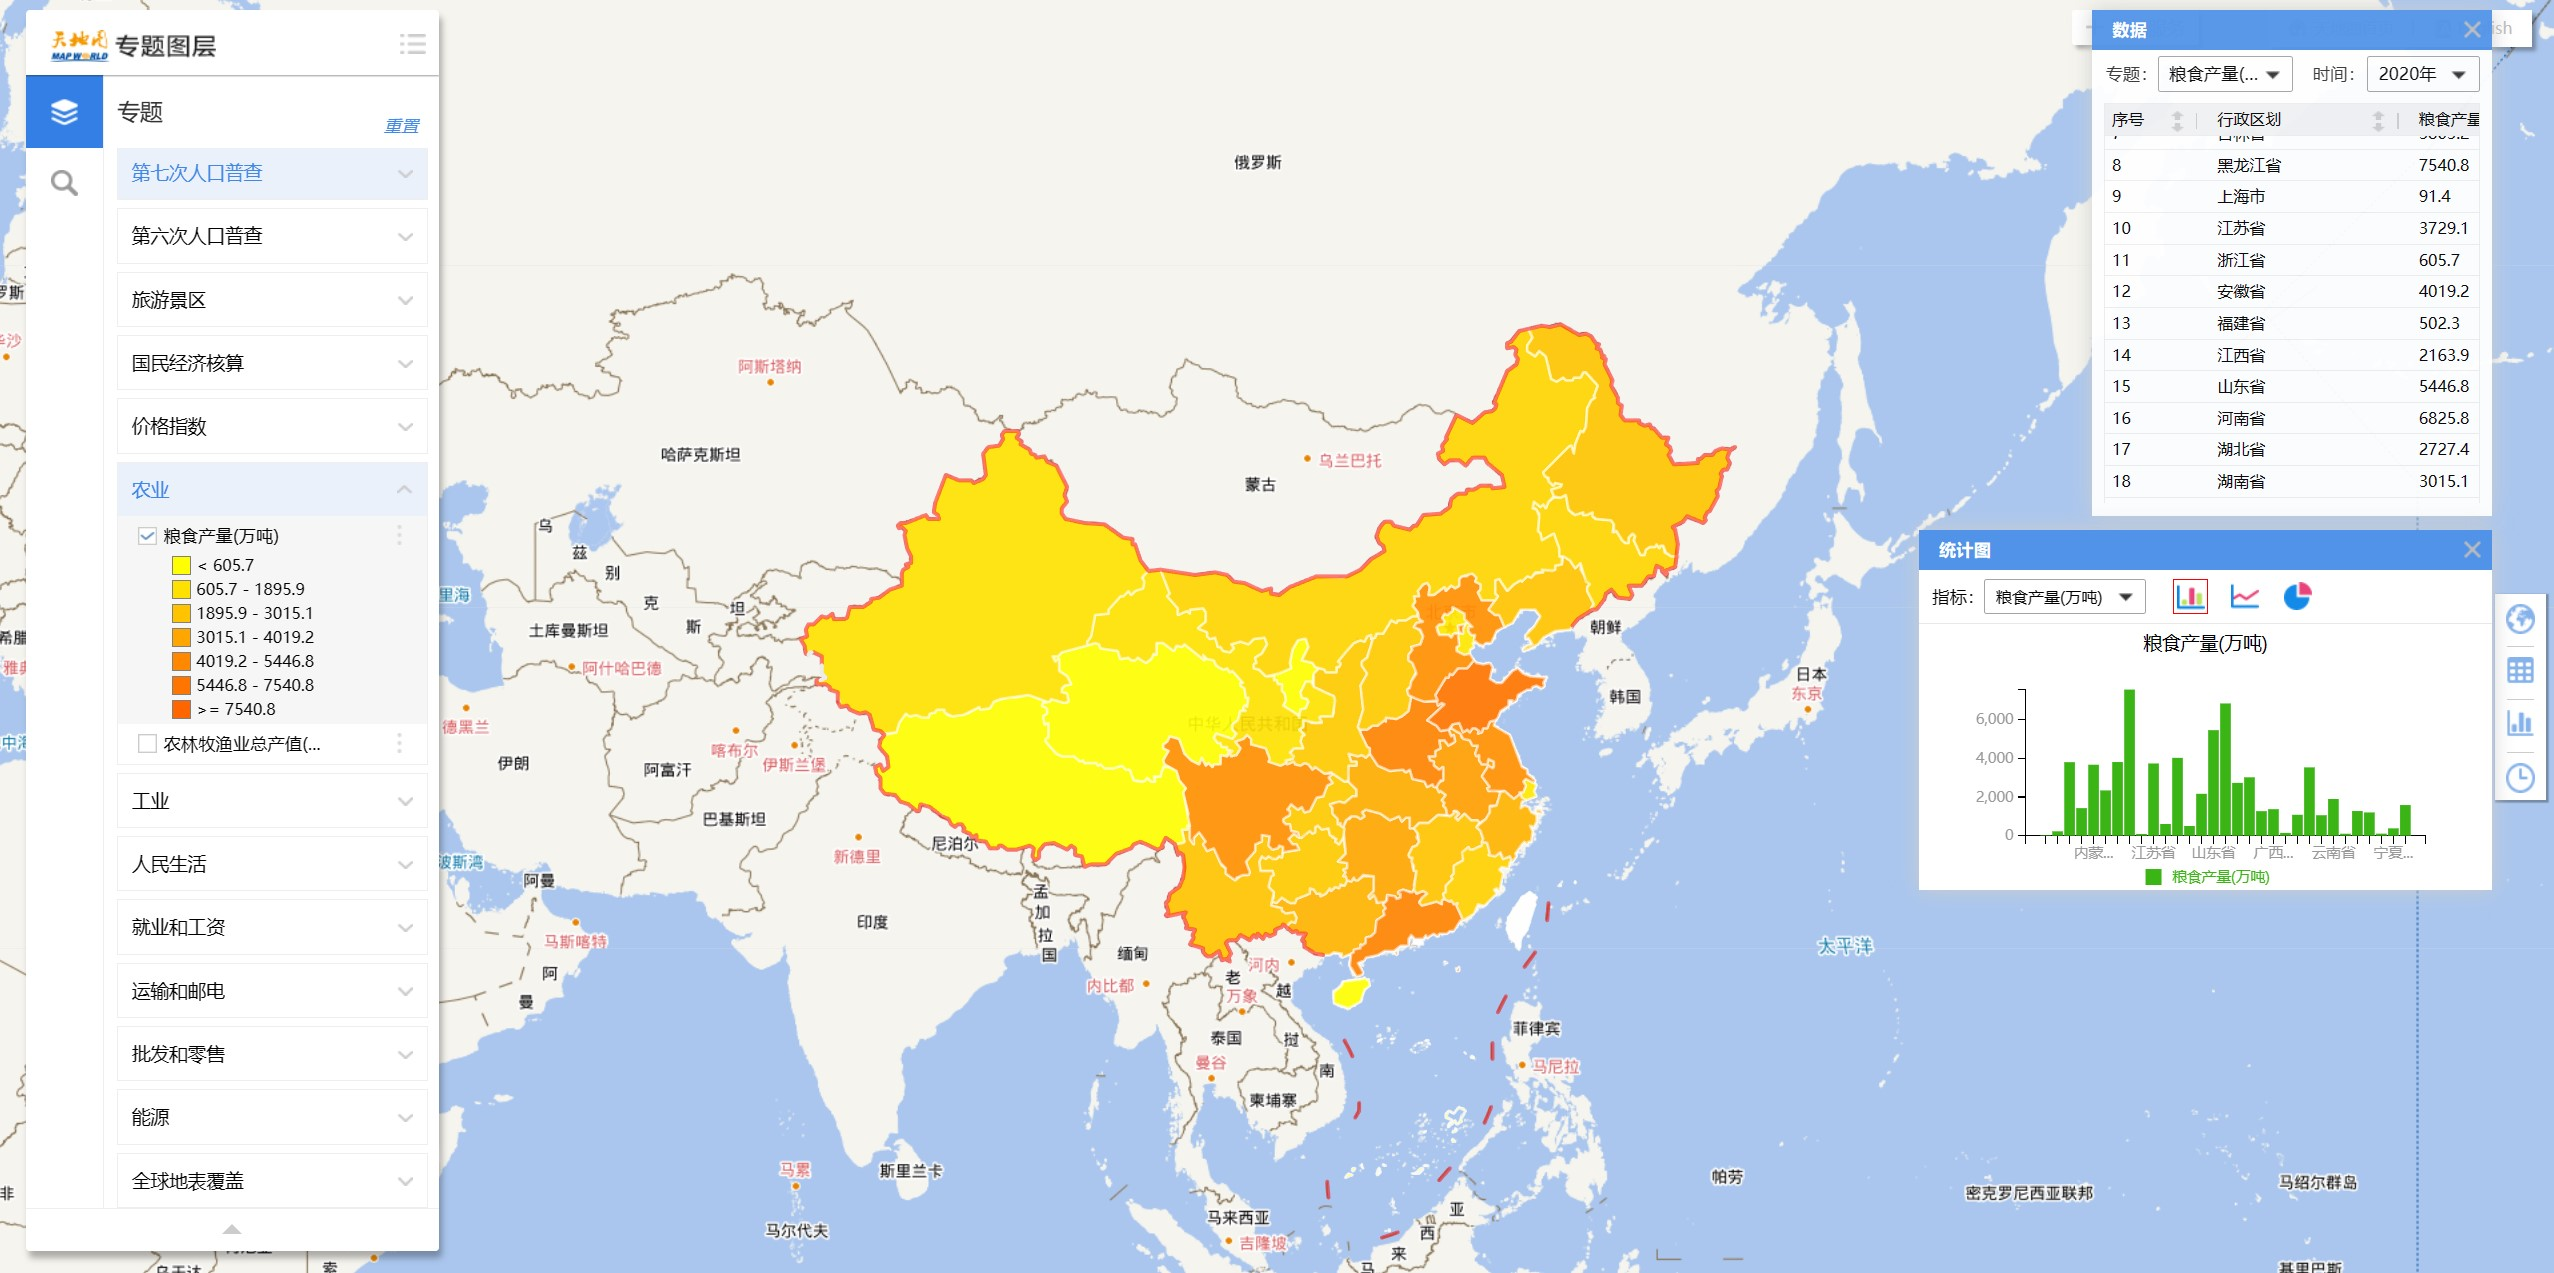
\includegraphics[height=.44\linewidth]{images/粮食产量}
    \end{figure}
\end{frame}

\begin{frame}
    \frametitle{第七次人口普查}
    \begin{figure}[htpb]
        \centering
        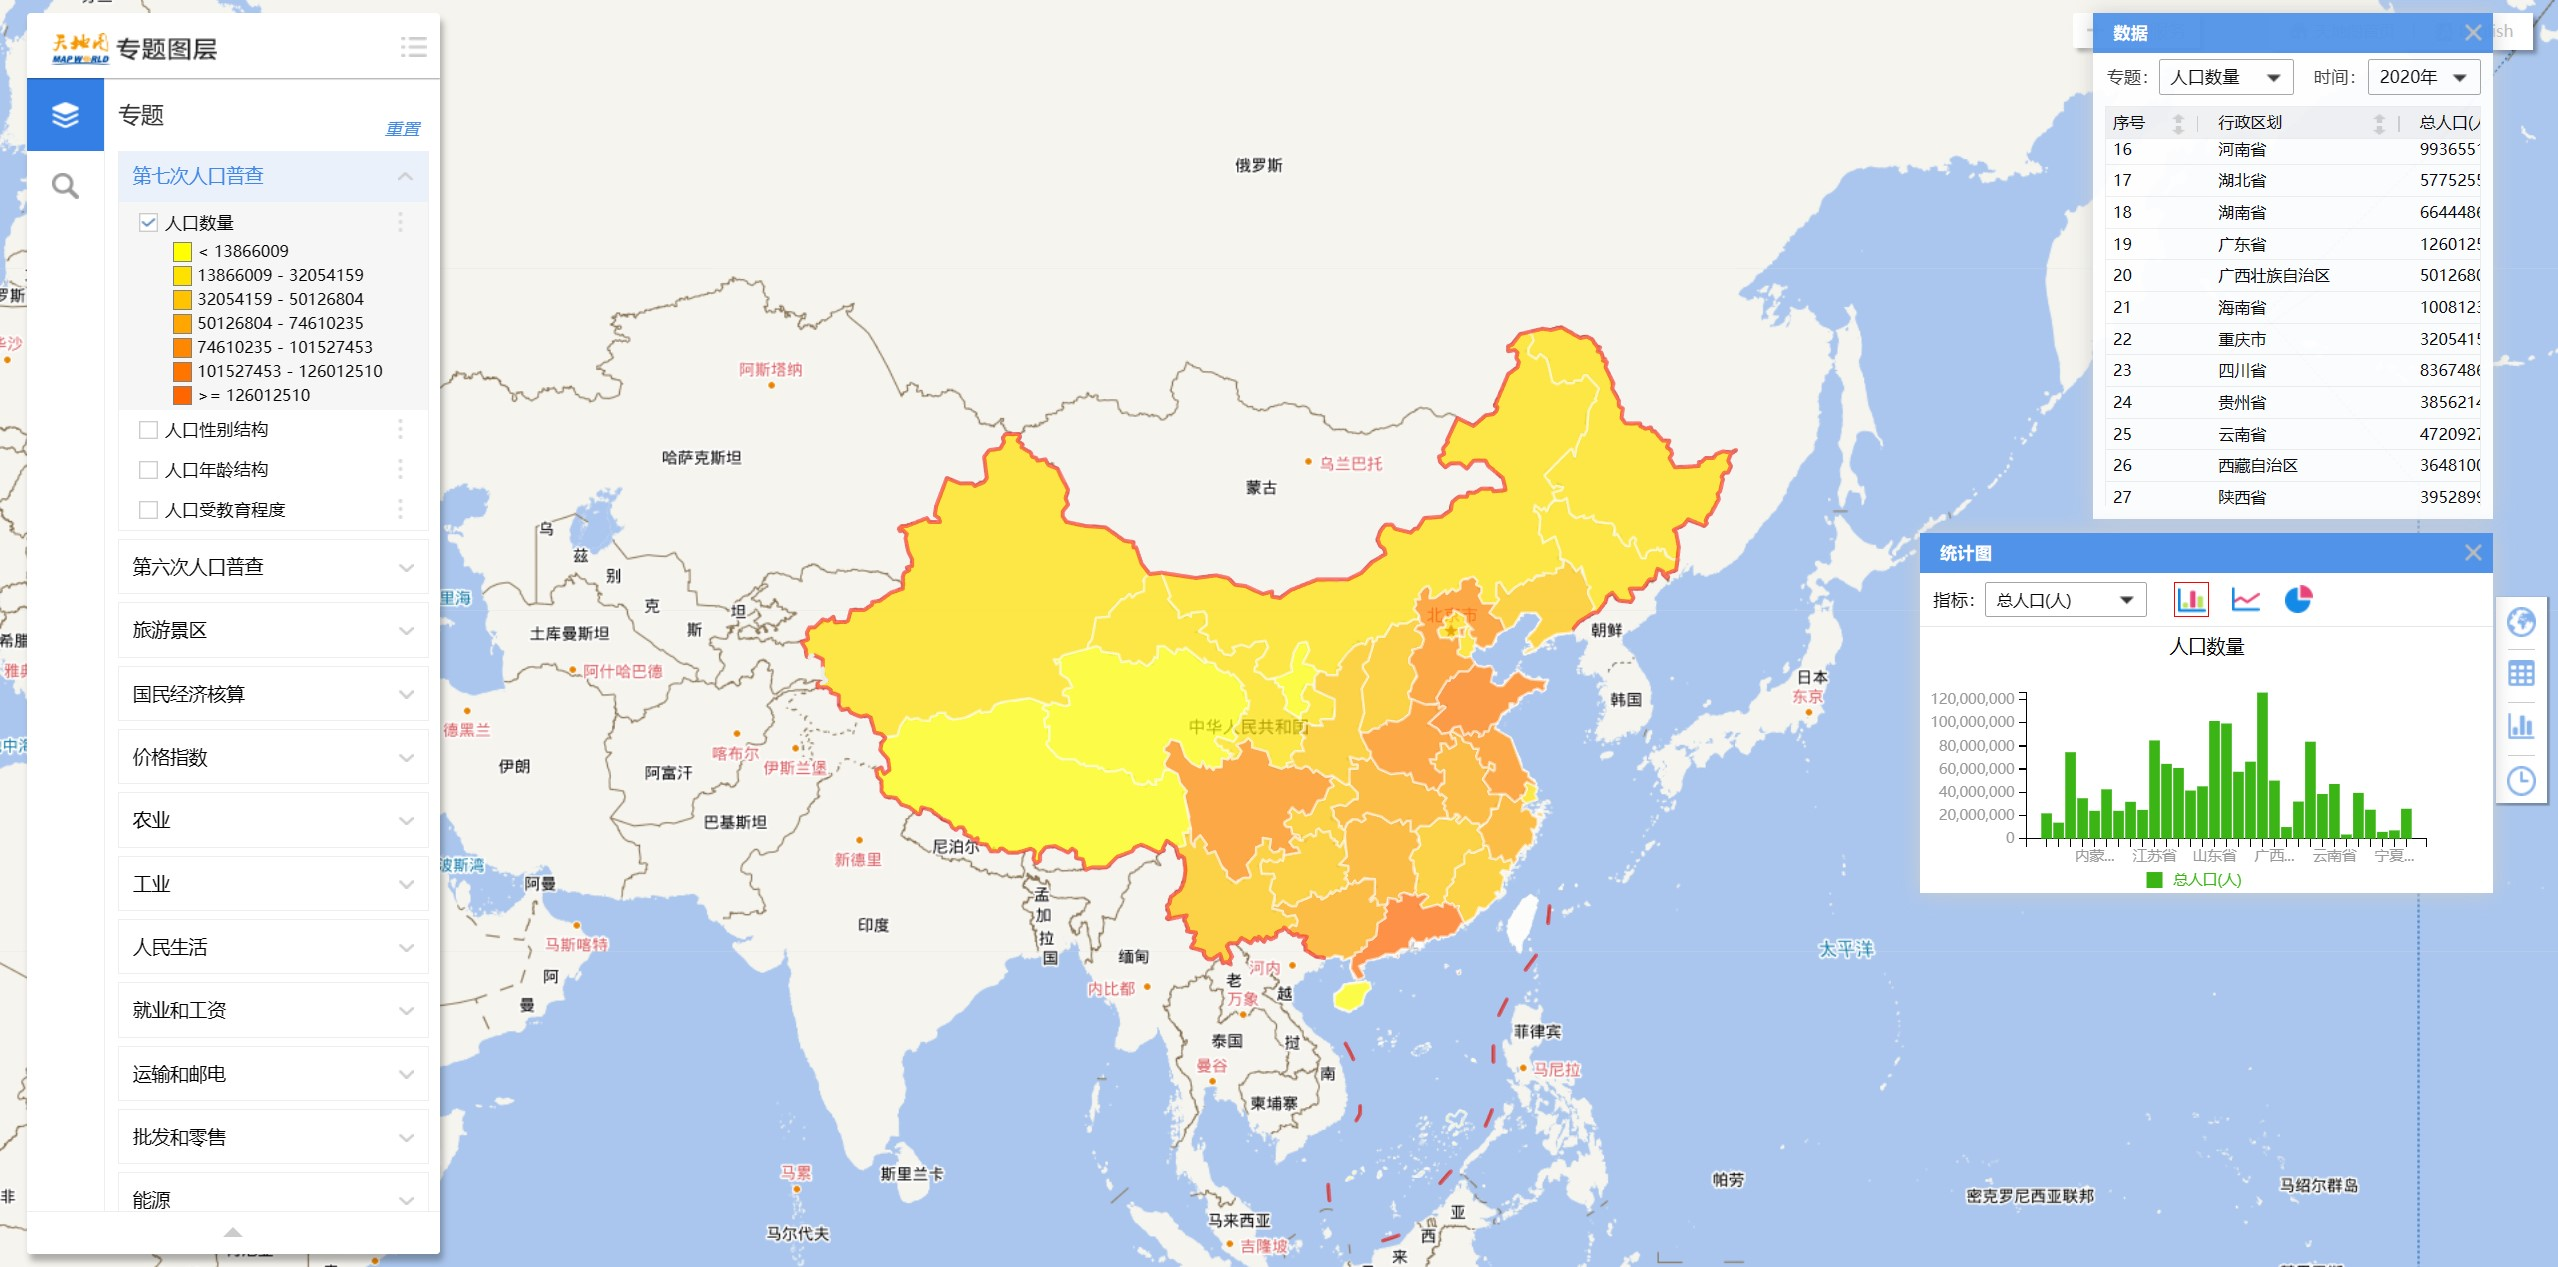
\includegraphics[height=.42\linewidth]{images/人口普查}
    \end{figure}
\end{frame}


\begin{frame}
    \frametitle{GPS与GIS的集成与应用}
    利用GIS中的电子地图和GPS接收机的实时差分定位技术，可以组成GPS+GIS的各种自动电子导航系统，也可以利用GPS的方法对GIS进行实时更新。
    \begin{itemize}
      \item 交通指挥调度
      \item 公安侦破
      \item 车船自动驾驶
      \item 农田作业管理
      \item 渔船捕鱼
    \end{itemize}
\end{frame}


\begin{frame}
    \frametitle{RS与GIS的集成与应用}
    RS是GIS重要的数据源和数据更新的手段，而反过来，GIS则是遥感中数据处理的辅助信息。两者集成可用于：
    \begin{itemize}
      \item 全球变化监测
      \item 农业收成面积监测
      \item 产量预估
      \item 空间数据自动更新
    \end{itemize}
\end{frame}


\begin{frame}
    \frametitle{GPS与RS的集成与应用}
    在遥感平台上安装GPS可以记录传感器在获取信息瞬间的空间位置数据，直接用于空三平差加密，可以大大减少野外控制测量的工作量。
    \begin{itemize}
      \item 自动定时数据采集
      \item 环境监测
      \item 灾害预测
    \end{itemize}

\end{frame}

\begin{frame}
    \frametitle{3S技术在农业中的应用}
        \begin{minipage}{0.68\linewidth}
            \begin{itemize}
                \item {\cbf{农田信息可视化}}
                
                通过各种离散空间数据的采集和GPS传感器的计算，完成对各种田间信息图形化处理。如病虫灾害覆盖图、耕地地力等级图、农作物产量分布图以及农业气候区划图等。
                \item {\cbf{农业生态环境研究}}
                
                地理信息系统广泛应用于农业生态环境研究的多个场景，包括环境监测、生态环境质量评价与环境影响评价、环境预测规划与生态管理以及面源污染防治等。
              \end{itemize}
        \end{minipage}\hfill
        \begin{minipage}{0.28\linewidth}
            \begin{figure}[htpb]
                \centering
                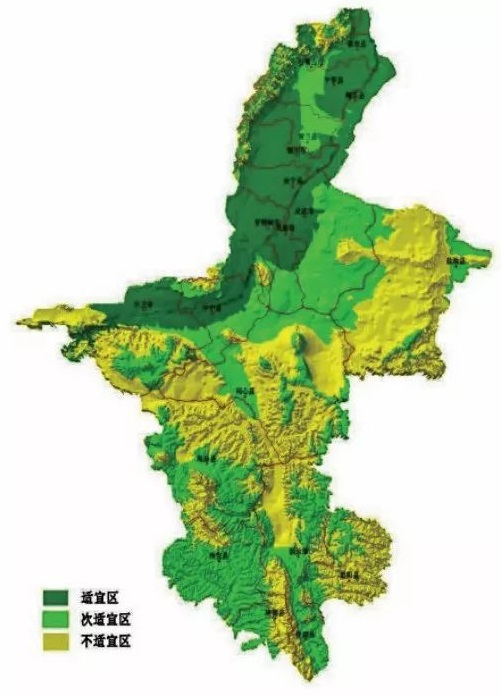
\includegraphics[width=\linewidth]{images/宁夏春小麦气候区划图}
                \caption{宁夏春小麦气候区划图}
            \end{figure}
        \end{minipage}
    
\end{frame}

\begin{frame}
    \frametitle{3S技术在农业中的应用}
    \begin{figure}[htpb]
        \centering
        \setcounter{subfigure}{0}
        \subfloat[土壤采样]{
\includegraphics[height=3cm]{土壤采样}}\hfill
        \subfloat[农田三维地形测量]{
\includegraphics[height=3cm]{农田三维地形测量}}\hfill
        \subfloat[农作物不同生育期长势监测]{
\includegraphics[height=3cm]{长势监测}}
    \end{figure}
\end{frame}

\begin{frame}
    \frametitle{3S技术集成应用-农业无人机 \link{https://ag.dji.com/cn/t50}}
        \begin{minipage}{0.58\linewidth}
            \begin{center}
                {\bfseries 智慧农业生态系统}
            \end{center}
            通过大疆智慧农业平台和全新 Mavic 3M 航测无人机，即可实现自动巡田、土地平整监测、出苗识别、长势分析、处方图变量作业等智慧农业解决方案。依据作物生长情况，结合农田处方图，农业无人飞机即可实现精准变量作业，如水稻变量施肥，棉花变量化控，大豆、玉米变量营养液等。
        \end{minipage}\hfill
        \begin{minipage}{0.38\linewidth}
            \begin{figure}[htpb]
                \centering
                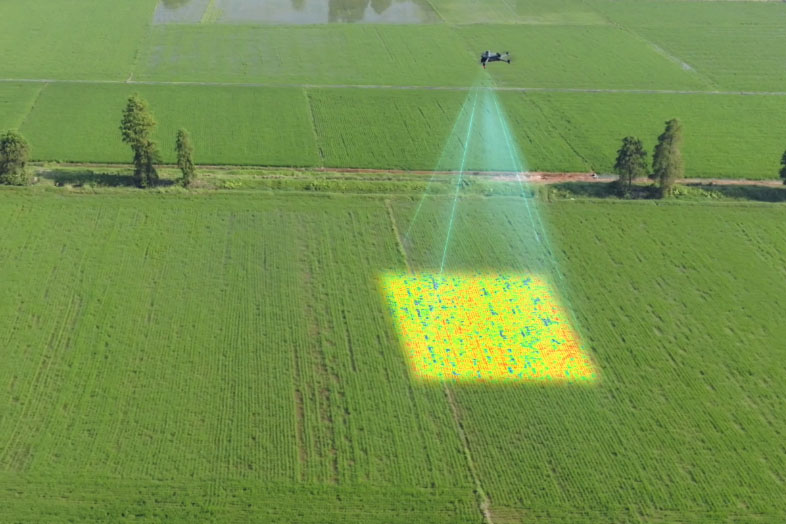
\includegraphics[width=.8\linewidth]{images/Mavic航测} 
                
                ~~~

                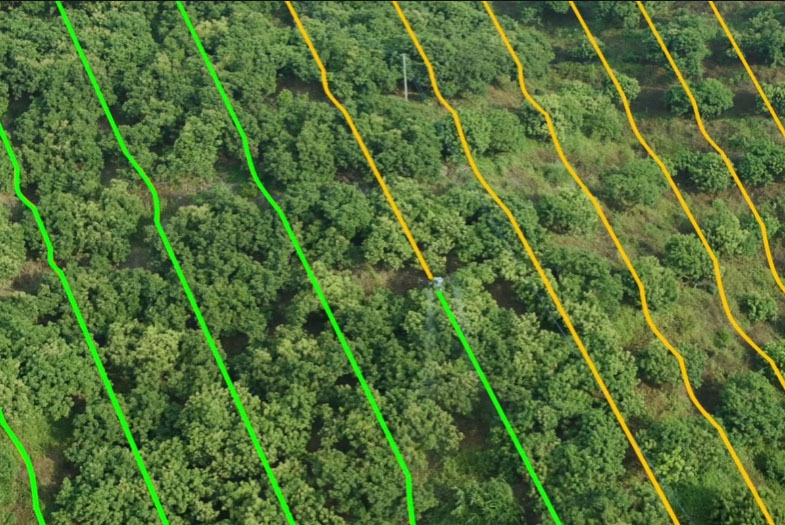
\includegraphics[width=.8\linewidth]{images/Mavic作业}
            \end{figure}
        \end{minipage}
    
\end{frame}


\begin{frame}
    \frametitle{农田测绘：从脚步丈量到无人机测绘}
    \begin{figure}[htpb]
        \centering
        \setcounter{subfigure}{0}
        \subfloat[脚步丈量，携带GPS手持测绘器采集边界的经纬坐标，利用计算机获取农田面积、地理位置等数据信息。]{
\includegraphics[height=3.8cm]{脚步丈量}}\hfill
        \subfloat[无人机测绘，搭载高精度 GNSS RTK 定位模块，航测精度达到了厘米级。]{
\includegraphics[height=3.8cm]{无人机测绘}}
    \end{figure}
\end{frame}


\subsection{条码技术}



\begin{frame}
    \frametitle{条码技术}
    条码技术是在计算机应用和实践中产生并发展起来的广泛应用于商业、邮政、图书管理、仓储、工业生产过程控制、交通等领域的一种自动识别技术，具有输入速度快、准确度高、成本低、可靠性强等优点，在当今的自动识别技术中占有重要的地位。
    \begin{figure}[htpb]
        \centering
        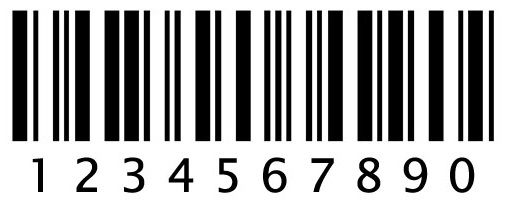
\includegraphics[height=.18\linewidth]{images/一维条码} \qquad 
        
\includegraphics[height=.22\linewidth]{images/二维码}
    \end{figure}
\end{frame}


\begin{frame}
    \frametitle{一维条码}
    一维条码是由一组规则排列的条、空以及对应的字符组成的标记，\maincolor{“条”指对光线反射率较低的部分，“空”指对光线反射率较高的部分}，这些条和空组成的数据表达一定的信息，并能够用特定的设备识读，转换成与计算机兼容的二进制和十进制信息。通常对于每一种物品，它的编码是唯一的。
    \begin{block}{说一说}
        你在哪些地方见过这样的条码？
        \begin{figure}[htpb]
            \centering
            
\includegraphics[width=.45\linewidth]{一维条码}
        \end{figure}
    \end{block}
\end{frame}


\begin{frame}
    \frametitle{工作原理}        
        \begin{minipage}{0.68\linewidth}
            由于不同颜色的物体，其反射的可见光的波长不同，白色物体能反射各种波长的可见光，黑色物体则吸收各种波长的可见光。条形码扫描仪则是一个可以发射可见光和接收其反射信号的仪器。在读取条形码的时候，它先向条形码发射一组可见光，这一组光照到条形码上，再反射给扫描仪上面的接收器，接收器根据其反射回来的光信号的强弱来识别条形码上的“条”、“空”信息。这些信息组合在一起，最终得到一组数字。
        \end{minipage}\hfill
        \begin{minipage}{0.28\linewidth}
            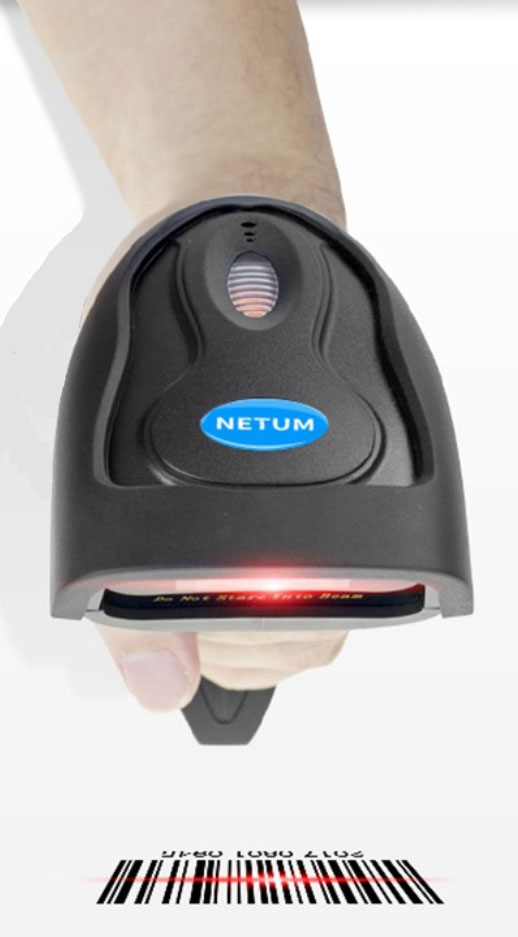
\includegraphics[height=180pt]{images/扫码枪}
        \end{minipage}
\end{frame}


\begin{frame}
    \frametitle{条码技术的特点}
    \begin{enumerate}
      \item 简单
      \item 信息采集速度快
      \item 采集信息量大
      \item 可靠性高
      \item 灵活、实用
      \item 自由度大
      \item 设备结构简单、成本低
    \end{enumerate}
\end{frame}


\begin{frame}
    \frametitle{POS系统}
    POS系统是通过读取产品的EAN码，在超市、便利店里管理销售、仓储和采购的系统。由于该系统也可以提供有关消费者需求趋向的准确资料，可以用来决策管理策略。

    \begin{figure}[htpb]
        \centering
        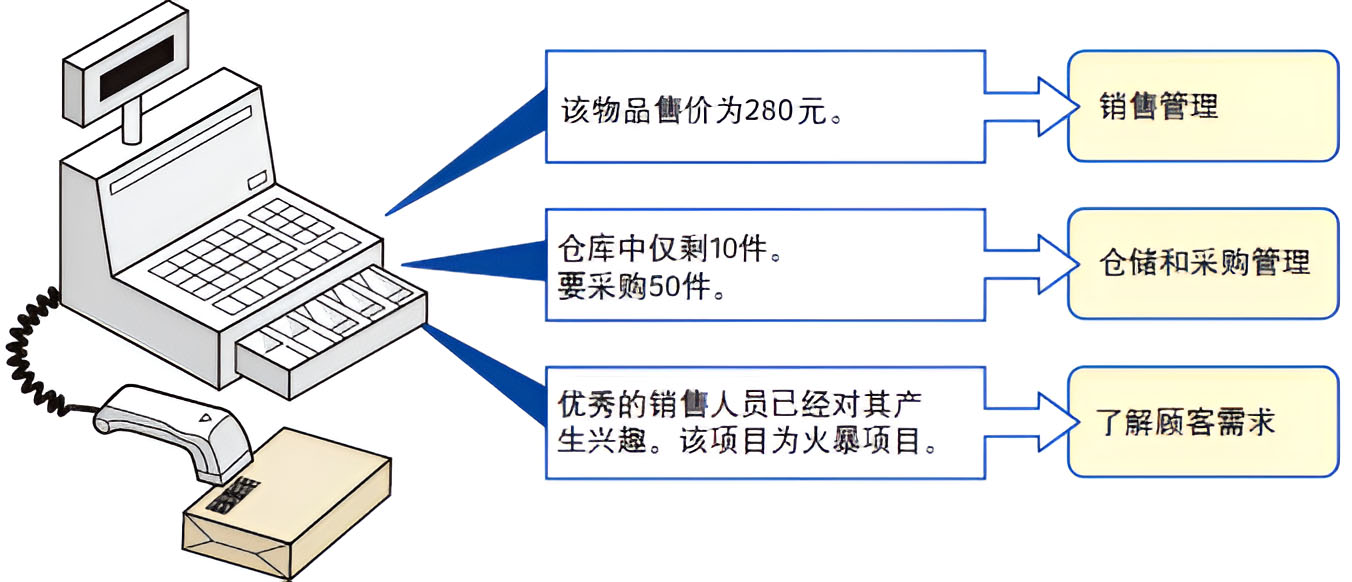
\includegraphics[height=.3\linewidth]{images/POS系统}
    \end{figure}
\end{frame}

\begin{frame}
    \frametitle{EAN码}
    EAN码（European Article Number）是国际物品编码协会制定的一种商品用条码，通用于全世界。EAN码有标准版（EAN-13）和缩短版（EAN-8）两种。
    
    国际条码组织给我国分配的编码从690到699。

    以690、691开头时，厂商识别码为四位，商品项目代码为五位；

    以692、693开头时，厂商识别码是五位，商品项目代码是四位。

    厂商识别代码: 由中国物品编码中心统一向厂商进行分配。

    商品项目代码:由厂商根据有关规定自行分配。

    \begin{figure}[htpb]
        \centering
        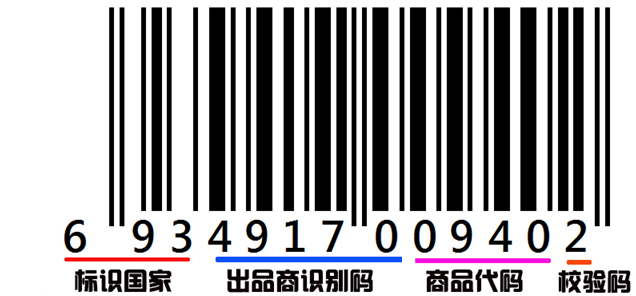
\includegraphics[height=.18\linewidth]{images/EAN码}
    \end{figure}
\end{frame}

\begin{frame}
    \frametitle{国际标准书号ISBN}
        \begin{minipage}{0.38\linewidth}
            \begin{figure}[htpb]
                \centering
                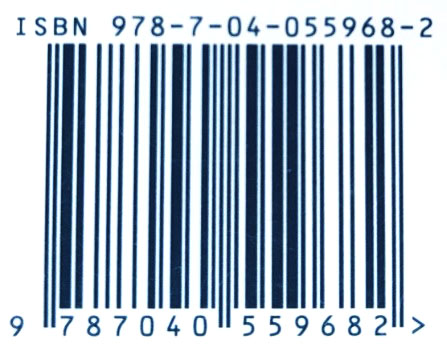
\includegraphics[height=.7\linewidth]{images/ISBN}
            \end{figure}
        \end{minipage}\hfill
        \begin{minipage}{0.58\linewidth}
            \begin{itemize}
              \item {\bfseries 978} \quad \ \,EAN图书码
              \item {\bfseries 7} \qquad ~\,地区码，7代表中国
              \item {\bfseries 04} \qquad 出版社代码，04为高等教育出版社
              \item {\bfseries 055968} 出版社的图书编号
              \item {\bfseries 2} \qquad ~\,校验码
            \end{itemize}
        \end{minipage}    
\end{frame}

% 2007年1月1日之前，ISBN由10位数字组成，分四个部分：组号（国家、地区、语言的代号），出版者号，书序号和检验码。2007年1月1日起，实行新版ISBN，新版ISBN由13位数字组成，分为5段，即在原来的10位数字前加上3位EAN图书产品代码“978”。最后一位重新校验。
% 前缀 978 989 图书，977期刊
% 第一组号码是国家代码（State Identifier），最短的是一位数字，最长的达五位数字，大体上兼顾文种、国别和地区。把全世界自愿申请参加国际标准书号体系的国家和地区，划分成若干地区，各有固定的编码：美国所出版的书国家代码为0，1代表英语，使用这两个代码的国家有：澳大利亚、加拿大、爱尔兰、新西兰、波多黎各、南非、英国、美国、津巴布韦等；2代表法语，法国、卢森堡以及比利时、加拿大和瑞士的法语区使用该代码；3代表德语，德国、奥地利和瑞士德语区使用该代码；4是日本出版物的代码；5是俄语系国家出版物的代码；7为中国大陆出版物使用的代码等等。国家领域最长可能为5位数字（如不丹为99936），但相对剩下能使用、分配的位数就较为狭隘。
% 第二组号码段
% 第二组号码是出版社代码（Publisher Identifier），由其隶属的国家或地区ISBN中心分配，允许取值范围为2-5位数字。出版社的规模越大，出书越多，其号码就越短。
% 第三组号码段
% 第三组号码是书序码（Title Identifier）由出版社自己给出，而且每个出版社的书序号是定长的（数字9，减去组号、出版社代码所占的位数，就是书序码的位数）。最短的一位，最长的六位。出版社的规模越大，出书越多，书序码越长（如人民文学出版社的出版社代码为02，书序码即为6位，译林出版社代码5447，书序码即为4位）。
% 第四组号码段
% 第四组号码是校验码，其数值由前九位数字依次以10～2加权之和并以11为模计算得到。


\begin{frame}
    \frametitle{条形码的读取}
    条码的黑色条表示二进制的1，白色代表0，而且0.33mm宽度的黑色或者白色条为一个基本的二进制位。有的黑白色条很宽，说明连着好几个二进制1/0。
    \begin{figure}[htpb]
        \centering
        
\includegraphics[width=.48\linewidth]{条形码读取1}
        
\includegraphics[width=.48\linewidth]{条形码读取2}
    \end{figure}
\end{frame}


\begin{frame}
    \frametitle{为什么同一个数字，条码不一样？}
    \qquad EAN码中，每个数字由7个二进制位组成，用黑条代表二进制1，白条代表0。每个数字的二进制表示方法有三个子集：A、B和C。    
\begin{table}[]
    \begin{tabular}{@{}cccccccc@{}}
    \toprule
               & \textbf{A 子集} & \textbf{B 子集} & \textbf{C 子集} & \textbf{}  & \textbf{A 子集} & \textbf{B 子集} & \textbf{C 子集} \\ \midrule
    \textbf{0} & 0001101       & 0100111       & 1110010       & \qquad \textbf{5} & 0110001       & 0111001       & 1001110       \\
    \textbf{1} & 0011001       & 0110011       & 1100110       & \qquad \textbf{6} & 0101111       & 0000101       & 1010000       \\
    \textbf{2} & 0010011       & 0011011       & 1101100       & \qquad \textbf{7} & 0111011       & 0010001       & 1000100       \\
    \textbf{3} & 0111101       & 0100001       & 1000010       & \qquad \textbf{8} & 0110111       & 0001001       & 1001000       \\
    \textbf{4} & 0100011       & 0011101       & 1011100       & \qquad \textbf{9} & 0001011       & 0010111       & 1110100       \\ \bottomrule
    \end{tabular}
    \end{table}
    \qquad 每个数字由两条黑条和两条白条构成，不同宽度的条代表连续的几个0或1。
\end{frame}

\begin{frame}
    \frametitle{根据前置码确定各个数字的编码}
    EAN-13商品条码中的前置码不用条码字符表示。左侧数据符选用A子集还是B子集取决于前置码的数值。右侧数据符及校验符均用字符集中的C子集表示。之所以这样规定，就是可以判断扫描正反，防止扫描错误。
    \bigskip

        \begin{minipage}{0.38\linewidth}
            \begin{figure}[htpb]
                \centering
                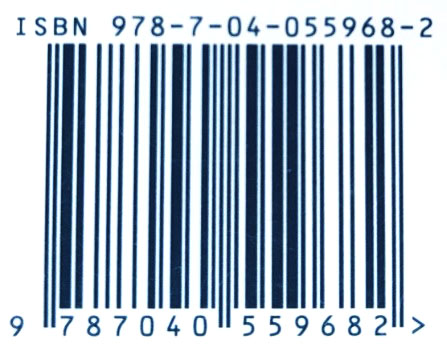
\includegraphics[width=\linewidth]{images/ISBN}
            \end{figure}
        \end{minipage}\hfill
        \begin{minipage}{0.58\linewidth}
            \smallskip

            \begin{table}[]
                \begin{tabular}{@{}ccccccccccc@{}}
                \toprule
                \textbf{前置码} & \textbf{0} & \textbf{1} & \textbf{2} & \textbf{3} & \textbf{4} & \textbf{5} & \textbf{6} & \textbf{7} & \textbf{8} & \textbf{9} \\ \midrule
                \textbf{左1}  & A          & A          & A          & A          & A          & A          & A          & A          & A          & A          \\
                \textbf{左2}  & A          & A          & A          & A          & B          & B          & B          & B          & B          & B          \\
                \textbf{左3}  & A          & B          & B          & B          & A          & B          & B          & A          & A          & B          \\
                \textbf{左4}  & A          & A          & B          & B          & A          & A          & B          & B          & B          & A          \\
                \textbf{左5}  & A          & B          & A          & B          & B          & A          & A          & A          & B          & B          \\
                \textbf{左6}  & A          & B          & B          & A          & B          & B          & A          & B          & A          & A          \\ \bottomrule
                \end{tabular}
                \end{table}
        \end{minipage}

\end{frame}


\begin{frame}
    \frametitle{Code 39，Code 128}
    \qquad 目前国内企业内部自定义码制，可以根据需要确定条码的长度和信息，它编码的信息可以是数字，也可以包含字母，广泛应用在企业内部管理、生产流程、物流控制系统等方面。

    \qquad Code 39 码，是目前 用途广泛的一种条形码，可表示数字、英文字母以及“−”、“.”、“/”、“+”、“\%”、“\$”、 “\ ”（空格）和“*”共 44 个符号，其中“*”仅作为起始符和终止符。

    \qquad CODE128 码可表示从 ASCII 0 到ASCII 127 共128个字符，故称128码。其中包含了数字、字母和符号字符。
    \begin{figure}[htpb]
        \centering
        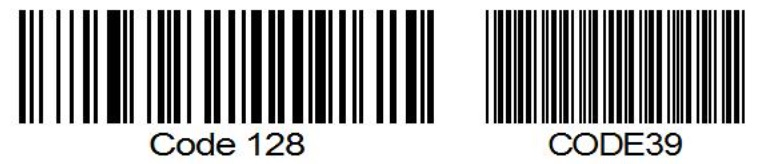
\includegraphics[width=.78\linewidth]{images/code128}
    \end{figure}
\end{frame}


\begin{frame}
    \frametitle{二维码}
        \begin{minipage}{0.58\linewidth}
            二维码是条形码的升级，条形码是一维，记录横向信息，不记录纵向。而二维码既记录横向也记录纵向。二维码能在有限的空间内存储更多的信息，并可脱离计算机使用。

            二维码是现在应用最广泛，最受青睐的标签，二维码的应用场景非常多，如对产品进行追溯、通过二维码进行保密管理、通过二维码读取文字信息、条码信息、产品出入库管理、产品防伪等等。
        \end{minipage}\hfill
        \begin{minipage}{0.38\linewidth}
            \begin{figure}[htpb]
                \centering
                
\includegraphics[width=\linewidth]{images/二维码}
            \end{figure}
        \end{minipage}
    
\end{frame}

\begin{frame}
    \frametitle{二维码的种类}
    \begin{itemize}
      \item 矩阵式二维码：Aztec、Maxi Code、QR Code、 Data Matrix等。
      \item 线性堆叠式二维码：Code 16K、Code 49、PDF417等。
    \end{itemize}
    \begin{figure}[htpb]
        \centering
        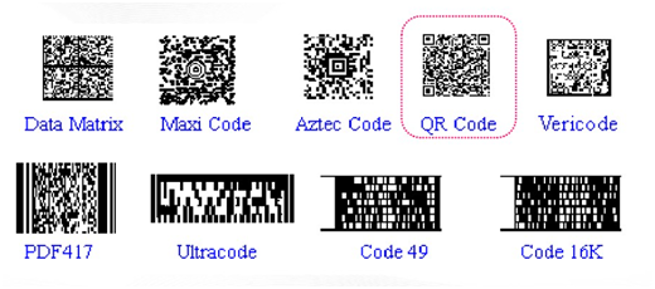
\includegraphics[height=.3\linewidth]{images/二维码种类}
    \end{figure}
\end{frame}

\begin{frame}
    \frametitle{QR码的规格}
    QR码设有1到40的不同版本(种类)，每个版本都具备固有的码元结构(码元数)。

    “码元结构”是指二维码中的码元数。从版本1(21码元×21码元)开始，在纵向和横向各自以4码元为单位递增，一直到版本40(177码元×177码元)。

    \begin{figure}[htpb]
        \centering
        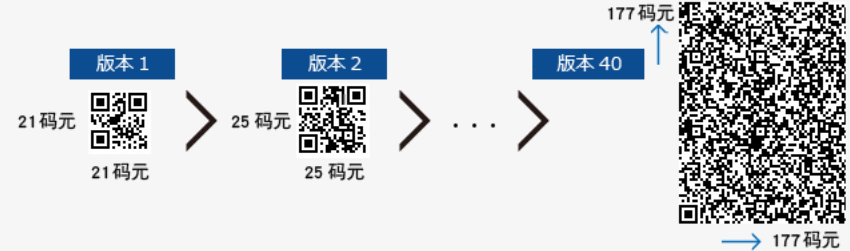
\includegraphics[width=\linewidth]{images/QR码的版本规格尺寸}
    \end{figure}
\end{frame}

\begin{frame}
    \frametitle{QR码的基本结构}
    \begin{figure}[htpb]
        \centering
        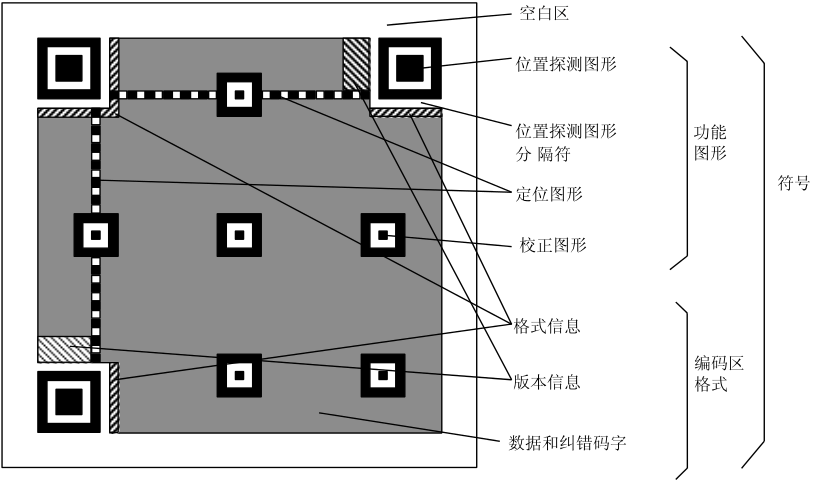
\includegraphics[height=.46\linewidth]{images/QR码的结构}
    \end{figure}
\end{frame}

\begin{frame}
    \frametitle{QR码的特点}
    \begin{itemize}
      \item 存储大容量信息
      \item 支持所有类型的数据
      \item 在小空间内打印
      \item 对变脏和破损的适应能力强
      \item 可以从任意方向读取
      \item 支持数据合并功能
    \end{itemize}
\end{frame}

% 传统的条形码只能处理20位左右的信息量，与此相比，QR码可处理条形码的几十倍到几百倍的信息量。

% 另外，QR码还可以支持所有类型的数据。（如：数字、英文字母、日文字母、汉字、符号、二进制、控制码等）。一个QR码最多可以处理7089字(仅用数字时)的巨大信息量。

% QR码使用纵向和横向两个方向处理数据，如果是相同的信息量，QR码所占空间为条形码的十分之一左右。(还支持Micro QR码，可以在更小空间内处理数据。)

% QR码从360°任一方向均可快速读取。其奥秘就在于QR码中的3处定位图案，可以帮助QR码不受背景样式的影响，实现快速稳定的读取。

% QR码可以将数据分割为多个编码，最多支持16个QR码。使用这一功能，还可以在狭长区域内打印QR码。另外，也可以把多个分割编码合并为单个数据。



\begin{frame}
    \frametitle{二维码应用}
            \begin{itemize}
              \item 移动支付
              \item 加好友，关注公众号
              \item 网站跳转
              \item 产品溯源
              \item 点餐购票
              \item 网站登录
              \item 广告促销
            \end{itemize}
\end{frame}


\begin{frame}
    \frametitle{农产品溯源系统}
    \begin{figure}[htpb]
        \centering
        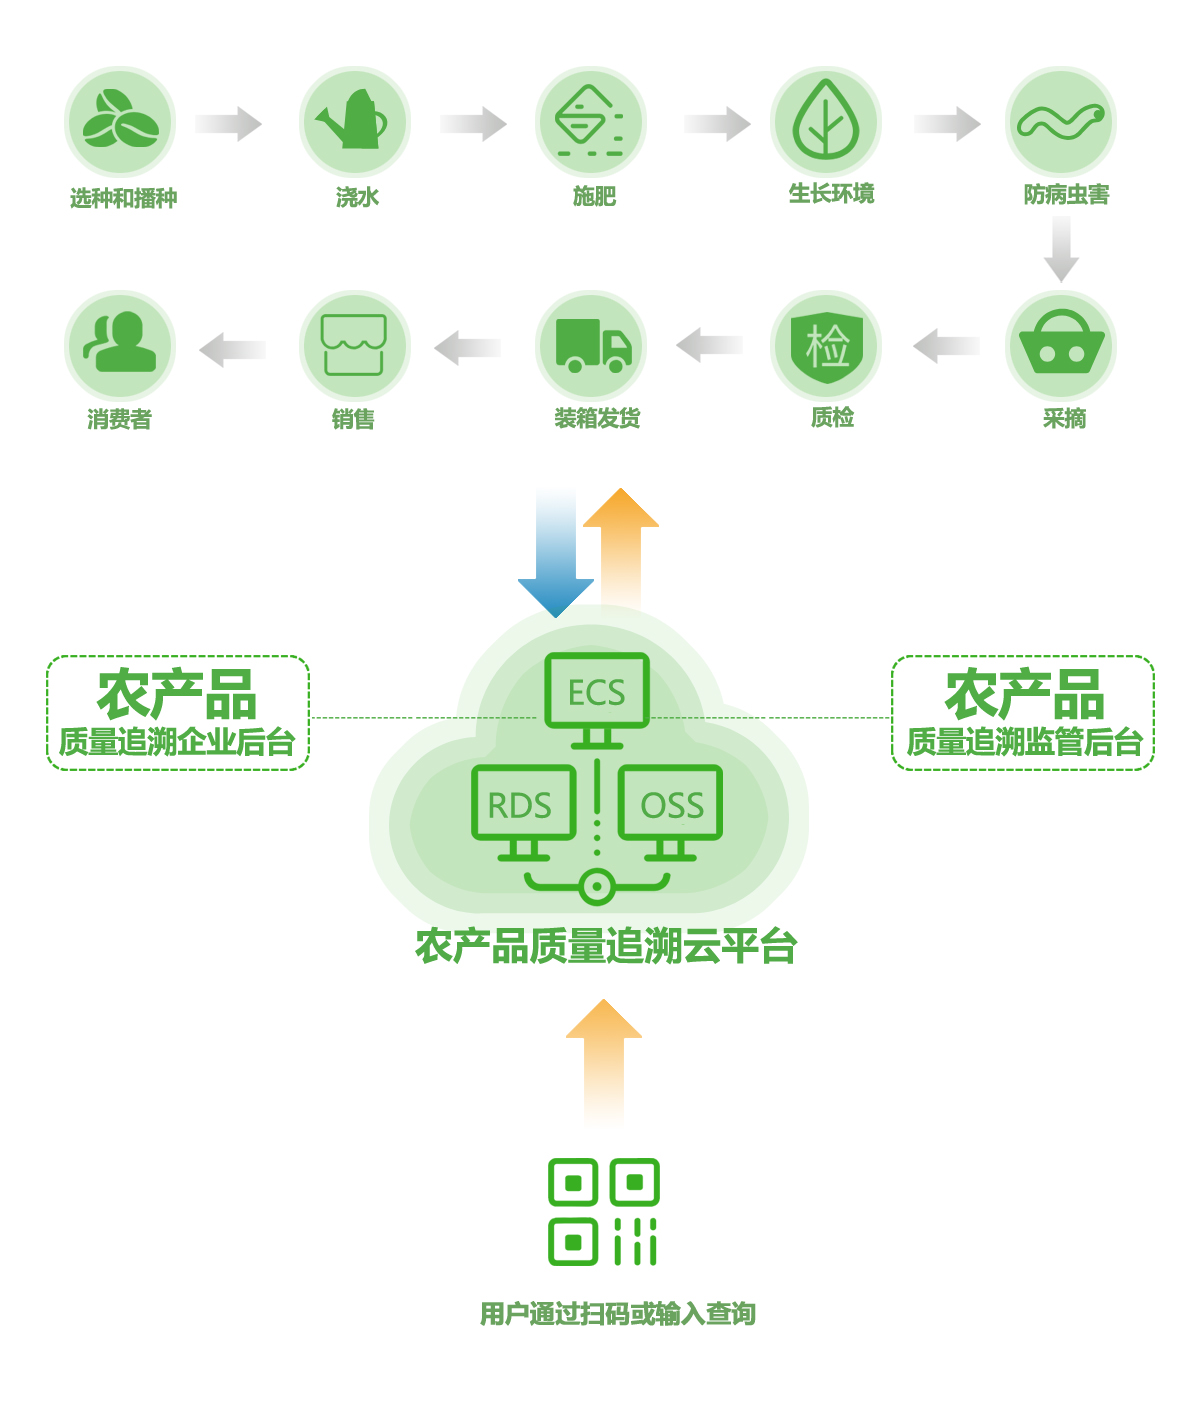
\includegraphics[height=.44\linewidth]{images/农产品溯源}
        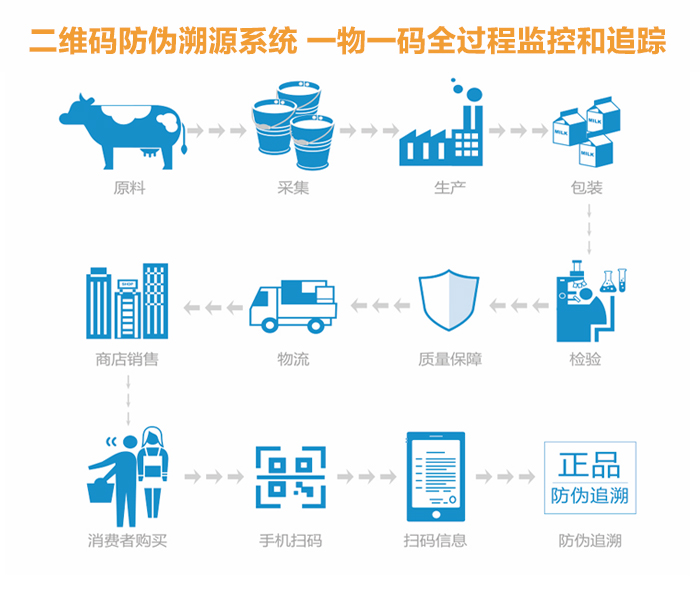
\includegraphics[height=.44\linewidth]{images/农产品溯源2}
    \end{figure}
\end{frame}


\subsection{种植养殖业数字化技术}

\begin{frame}
    \frametitle{种植业数字化技术}
    种植业数字化是数字技术在农作物种植各环节的应用，通过获取、记录农业生产经营各环节数据，并计算分析得出应对方案，为种植各环节流程提供智能决策，提高生产效率。
    \begin{itemize}
      \item {\cbf{数字化“三情”监测分析}} 利用物联网等信息化手段对墒情、苗情、灾情等“三情”和气象进行预测预报，精准指导生产决策。
      \item {\cbf{病虫害监测数字化}} 利用智能化监测设备、轨迹分析模型与数字化预测技术，建成全国统一的病虫害数字化监测预警平台。
      \item {\cbf{农田自动化生产管理}} 通过信息监测、信息分析、智能决策、自动控制等技术手段，实现农田的信息在线感知、精细生产管控、高效运维管理。
      \item {\cbf{数字农场建设}} 面向规模化种植基地和大型农场，依据不同种植品种、不同生产模式、不同区域条件进行农业机械和施肥灌溉设备等的智能化改造和集成应用。
    \end{itemize}

\end{frame}

\begin{frame}
    \frametitle{养殖业数字化技术}
    \begin{itemize}
      \item {\cbf{动物疫病监测数字化}} 利用网络数字技术、智能感知技术和监控设施设备对规模化养殖场进行疾病监测和疫病传播跟踪，提高动物疫病防控能力与处置效率。建立动物电子免疫档案，实现动物疫病强制免疫信息化管理。
      \item {\cbf{畜牧养殖监管数字化}} 对畜牧养殖过程进行全程监控，依托畜牧养殖大数据监管平台，记录全环节畜牧养殖流转信息，形成环环相扣的信息链条，有效防范不法分子违规开具检疫证明、违规调运等问题。
      \item {\cbf{数字牧场建设}} 通过对牧场（养殖场）全场设备数字化和网络化控制，收集环境指标、饲料消耗、环保指标等关键传感数据，实现畜禽养殖全过程的数据采集、数据分析、过程优化、智能控制和信息追溯，通过精细化养殖，提升效益。
    \end{itemize}

\end{frame}


\begin{frame}
    \frametitle{智慧养猪场}
    \begin{figure}[htpb]
        \centering
        
\includegraphics[width=.7\linewidth]{智慧养猪厂}
    \end{figure}
    \vspace{-2pt}
\end{frame}

% 智慧养猪场解决方案通过运用最新的物联网技术和RFID技术将养猪生产管理、猪舍环境监控、产品溯源、自动化控制系统整合为一套完整的系统，通过传感器检测猪舍中的环境，从而给猪提供舒适的温度和通风量，智慧养殖系统实现养猪科学化、制度化、信息化、精准化，带给养殖户更多的收益。


\begin{frame}
    \frametitle{智慧养殖系统的设计方案}
    \begin{figure}[htpb]
        \centering
        
\includegraphics[width=.8\linewidth]{智慧养殖方案}
    \end{figure}
\end{frame}



